% -*- root: main.tex -*-

\chapter{The \texorpdfstring{$\sigma$}{sigma}-orientation}\label{ChapterSigmaOrientation}

By this point, we have seen a great many ways that algebraic geometry exerts control over the behavior of homotopy theory, stable and unstable.  The goal in this Case Study is to explore a setting where algebraic geometry is itself tightly controlled: whereas the behavior of formal groups is quite open-ended, the behavior of \emph{abelian varieties} is comparatively strict.  We import this strictness into algebraic topology by stiudying complex-orientable cohomology theories $E$ which have been tagged with an auxiliary abelian variety $A$ via an isomorphism $\phi\co \CP^\infty_E \cong A^\wedge_0$.  In the case that $A$ is an elliptic curve, this is our definition of an \textit{elliptic cohomology theory}.  The idea, then, is not that this puts serious constraints on the formal group $\CP^\infty_E$ (although it does place some), but rather that the theory of abelian varieties endows $A$, and hence $A^\wedge_0$, with various bits of preferred data.  This is the tack we take to construct a \emph{canonical} $MU[6, \infty)$--orientation of $E$: for any complex-orientable $E$, we identify the collection of such ring maps with ``$\Theta$--structures on $\CP^\infty_E$''; a basic theorem about abelian varieties endows the elliptic curve $A$ with a canonical such structure; and altogether this yields the desired orientation for an elliptic spectrum.

Making the identification of $MU[6, \infty)$--orientations with $\Theta$--structures requires real work, but many of the stepping stones are now in place.  We begin with a technical section about especially nice formal schemes, called \textit{coalgebraic}, and we use this to finally give the proof, announced back in \Cref{DivConstructionsAreFree}, that the scheme of stable Weil divisors on a formal curve presents the free formal group on that curve.  With that out of the way and with $MU[6, \infty)$ in mind as the eventual goal, we then summarize the behavior of the part of the Postnikov tower for complex bordism that we \emph{do} understand---the cases of $MUP$ and $MU$---and use this to make an analysis of $MSU$.  In particular, we rely heavily on the results from \Cref{ComplexBordismChapter} and \Cref{ChapterFiniteSpectra} to understand the co/homological behaviors of $BU \times \Z$, $BU$, $MUP$, and $MU$.

The coherence of all of these statements gives us very explicit target theorems to aim for in our study of $MU[6, \infty)$, but we are forced to approach them from a different vantage point: whereas we can prove a splitting principle for $SU$--bundles, the analogous statement for $U[5, \infty)$--bundles does not appear to admit a direct proof.  Consequently, the proofs of the other structure theorems for $BU[6, \infty)$ and $MU[6, \infty)$ are made considerably more complicated because we have to work with our splitting principle hands tied.  Instead, our main tools are the results developed in \Cref{UnstableCooperationsChapter}, which give us direct access to the co/homology of the layers of the Postnikov tower.  When the dust of all this settles, we will have arrived at a very satisfying and complete theory of $MU[6, \infty)$--orientations, applicable to an arbitrary complex-orientable cohomology theory.

The reader gifted with an exceptional attention span will recall from the Introduction that we were \emph{really} interested in $M\String$--orientations, and that our interest in $MU[6, \infty)$--orientations was itself only a stepping stone.  We close this Case Study with an analysis of this last setting, where we finally yield and place more hypotheses on $E$---a necessity for gaining calculational access to co/homological behavior of objects like $B\String$, which lie outside of the broader complex-orientable story.

We also give a short r\'esum\'e on the theory of elliptic curves in \Cref{SectionEllipticCurvesAndThetaFunctions}, extracting the smallest possible subset of their theory that we will need here.









\section{Coalgebraic formal schemes}

We will now finally address an elephant that has been lingering in our metaphorical room: in the first third of this book we were primarily interested in the formal scheme associated to the \emph{cohomology} of a space, but in the second third we were primarily interested in a construction converting the \emph{homology} of a spectrum to a sheaf over a context.  Our goal for today is to, when possible, put these two variances on even footing.  Our motivation for putting this lingering discrepancy to rest is more technical than aesthetic: we have previously wanted access to certain colimits of formal schemes (e.g., in \Cref{DivConstructionsAreFree}).  While such colimits are generally forbidding, similarly to colimits of manifolds, we will in effect produce certain conditions under which they are accessible.

For $E$ a ring spectrum and $X$ a space, the diagonal map $\Delta\co X \to X \times X$ induces a multiplication map on $E$--cohomology via the composite \[E^* X \otimes_{E^*} E^* X \xrightarrow{\text{K\"unneth}} E^*(X \times X) \xrightarrow{E^* \Delta} E^* X.\]  Dually, applying $E$--homology, we have a pair of maps \[E_* X \xrightarrow{E_* \Delta} E_*(X \times X) \xleftarrow{\text{K\"unneth}} E_* X \otimes_{E_*} E_* X,\] where, remarkably, the K\"unneth map goes the wrong way to form a composite.  In the case that that map is an isomorphism, the long composite induces the structure of an $E_*$--coalgebra on $E_* X$.  In the most generous case that $E$ is a field spectrum (in the sense of \Cref{FieldSpectraAreKTheories}), the K\"unneth map is always invertible and, moreover, $E^* X$ is functorially the linear dual of $E_* X$.  This motivates us to consider the following purely algebraic construction:

\begin{definition}
Let $C$ be a coalgebra over a field $k$.  We define a functor
\begin{align*}
\Sch C\co \CatOf{Algebras}_{k/} & \to \CatOf{Sets}, \\
T & \mapsto \left\{f \in C \otimes T \middle| \begin{array}{c} \Delta f = f \otimes f \in (C \otimes T) \otimes_T (C \otimes T), \\ \eps f = 1 \end{array} \right\}.
\end{align*}
\end{definition}

\begin{lemma}
For a field $k$ and a $k$--algebra $A$ which is finite--dimensional as a $k$--module, there is a natural isomorphism $\Spec A \cong \Sch A^*$.
\end{lemma}
\begin{proof}[Proof sketch]
A point $f \in (\Sch A^*)(T) \subseteq A^* \otimes T$ gives rise to a $k$--module map $f_*\co A \to T$, which the extra conditions in the formation of $(\Sch C)(T)$ force to be a ring homomorphism.  The finiteness assumption is present exactly so that $A$ is its own double--dual, giving an inverse assignment.
\end{proof}

If we drop the finiteness assumption, then this comparison proof fails entirely.  Indeed, the multiplication on $A$ gives rise only to maps \[A^* \to (A \otimes_k A)^* \from A^* \otimes_k A^*,\] which is not enough to make $A^*$ into a $k$--coalgebra.  However, if we start instead with a $k$--coalgebra $C$ of infinite dimension, the following result is very telling:

\begin{lemma}[{\cite[pg.\ 12]{Demazure}, \cite[Appendix 5.3]{Michaelis}, \cite[Remark 1.1.8]{HopkinsLurie}}]\label{kCoalgebrasAreIndFinite}
For $C$ a coalgebra over a field $k$, any finite--dimensional $k$--linear subspace of $C$ can be finitely enlarged to a subcoalgebra of $C$.  Accordingly, taking the colimit gives a canonical equivalence
\[\pushQED{\qed}
\Ind(\CatOf{Coalgebras}_k^{\mathrm{fin}}) \xrightarrow{\simeq} \CatOf{Coalgebras}_k. \qedhere
\popQED\]
\end{lemma}

\noindent This result allows us to leverage our duality Lemma pointwise: for an arbitrary $k$--coalgebra, we break it up into a lattice of finite $k$--coalgebras, and take their linear duals to get a reversed lattice of finite $k$--algebras.  Altogether, this indicates that $k$--coalgebras generally want to model \emph{formal schemes}.

\begin{corollary}\label{CoalgsAndFSchsAgreeOverk}
For $C$ a coalgebra over a field $k$ expressed as a colimit $C = \colim_k C_k$ of finite subcoalgebras, there is an equivalence \[\Sch C \cong \{\Spec C_k^*\}_k.\]  This induces a \emph{covariant} equivalence of categories \[\CatOf{Coalgebras}_k \cong \CatOf{FormalSchemes}_{/k}.\]  This equivalence translates between the product of formal schemes, the tensor product of pro-algebras, and the tensor product of coalgebras. \qed
\end{corollary}

This covariant algebraic model for formal schemes is very useful.  For instance, this equivalence makes the following calculation trivial:
\begin{lemma}[{cf.\ \Cref{HF2BOIsSymAlg}, \Cref{DivConstructionsAreFree}, and \Cref{ECohomBUIsFree}}]
Select a coalgebra $C$ over a field $k$ together with a pointing $k \to C$.  Write $M$ for the coideal $M = C / k$.  The free formal monoid on the pointed formal scheme $\Sch k \to \Sch C$ is given by \[F(\Sch k \to \Sch C) = \Sch \Sym^* M.\]  Writing $\Delta c = \sum_j \ell_j \otimes r_j$ for the diagonal on $C$, the diagonal on $\Sym^* C$ is given by
\[\pushQED{\qed}
\Delta(c_1 \cdots c_n) = \sum_{j_1, \ldots, j_n} (\ell_{1,j_1} \cdots \ell_{n, j_n}) \otimes (r_{1, j_1} \cdots r_{n, j_n}). \qedhere
\popQED\]
\end{lemma}

It is unfortunate, then, that when working over a ring rather than a field \Cref{kCoalgebrasAreIndFinite} fails~\cite[Appendix 5.3]{Michaelis}.  Nonetheless, it is possible to bake into the definitions the machinery needed to get a good-enough analogue of \Cref{CoalgsAndFSchsAgreeOverk}.

\begin{definition}[{\cite[Definition 4.58]{StricklandFSFG}}]\label{DefnCoalgebraicFormalScheme}
Let $C$ be an $R$--coalgebra which is free as an $R$--module.  A basis $\{x_j\}$ of $C$ is said to be a \textit{good basis} when any finite subcollection of $\{x_j\}$ can be finitely enlarged to a subcollection that spans a subcoalgebra.  The coalgebra $C$ is itself said to be \textit{good} when it admits a good basis.  A formal scheme $X$ is said to be \textit{coalgebraic} when it is isomorphic to $\Sch C$ for a good coalgebra $C$.
\end{definition}

\begin{example}\label{FVarsAreCoalgebraic}
The formal scheme $\A^n$ is coalgebraic.  Beginning with the presentation \[\A^n = \Spf R\ps{x_1, \ldots, x_n} = \colim_J \Spec R[x_1, \ldots, x_n] / (x_1^{j_1}, \ldots, x_n^{j_n}),\] write $A_J$ for the algebra on the right-hand side.  Each $A_J$ is a free $R$--module, and we write \[C_J = A_J^* = R\{\beta_K \mid K < J\}\] for the dual coalgebra, with \[\beta_K(x^L) = \begin{cases} 1 & \text{if $K = L$}, \\ 0 & \text{otherwise}. \end{cases}\]  The elements $\beta_K$ form a good basis for the full coalgebra $C = \colim_J C_J$: any finite collection of them $\{\beta_K\}_{K \in \mathcal K}$ is contained inside any $C_J$ satisfying $K < J$ for all $K \in \mathcal K$.  As an additional consequence, all formal varieties are coalgebraic.
\end{example}

The main utility of this condition is that it gives us access to colimits of formal schemes:

\begin{theorem}[{\cite[Proposition 4.64]{StricklandFSFG}}]\label{CoalgebraicColimitsExist}
Suppose that $F\co \CatOf I \to \CatOf{Coalgebras}_R$ is a colimit diagram of coalgebras such that each object in the diagram, including the colimit point, is a good coalgebra.  Then \[\Sch \circ \, F\co \CatOf I \to \CatOf{FormalSchemes}\] is a colimit diagram of formal schemes. \qed
\end{theorem}

\noindent For an example of the sort of constructions that become available via this Theorem, we prove the following Corollary by analyzing the symmetric power of coalgebras:

\begin{corollary}[{\cite[Example 4.65 and Proposition 6.4]{StricklandFSFG}}]\label{ProofOfFreeFormalMonoids}
When a formal scheme $X$ is coalgebraic, the symmetric power $X^{\times n}_{\Sigma_n}$ exists.  In fact, $\coprod_{n \ge 0} X^{\times n}_{\Sigma n}$ models the free formal monoid on $X$.  Given an additional pointing $\Spec R \to X$, the colimit of the induced system \[\colim \left(\cdots \to X^{\times n}_{\Sigma_n} = \Spec R \times X^{\times n}_{\Sigma_n} \to X \times X^{\times n}_{\Sigma_n} \to X^{\times(n+1)}_{\Sigma_{n+1}} \to \cdots\right)\] models the free formal monoid on the pointed formal scheme.
\end{corollary}
\begin{proof}[Proof sketch]
The main points entirely mirror the case over a field: the symmetric power construction gives models for $X^{\times n}_{\Sigma_n}$, the symmetric algebra construction gives a model for the free formal monoid, and the stabilization against the pointing is modeled by inverting an element in the symmetric algebra.  In each case, choosing a good basis for the coalgebra underlying $X$ yields choices of good bases for the coalgebras arising from these constructions, essentially because their elements are crafted out of finite combinations of the elements of the original.
\end{proof}

In the specific case that $\Spec R \to X$ is a pointed formal \emph{curve}, we can prove something more:
\begin{corollary}[{\cite[Proposition 6.12]{StricklandFSFG}}]\label{FreeFormalGroupOnACurve}
For $\Spec R \to X$ a pointed formal curve, the free formal monoid is automatically an abelian group.
\end{corollary}
\begin{proof}[Proof sketch]
The main idea is that the coalgebra associated to a formal curve admits an increasing filtration $F_k$ so that the reduced diagonal $\overline \Delta = \Delta - (1 \otimes \eta) - (\eta \otimes 1)$ reduces filtration degree: \[\overline \Delta|_{F_k}\co F_k \to \sum_{\substack{i,j > 0 \\ i+j=k}} F_i \otimes F_j.\]  In turn, the symmetric algebra on the coalgebra associated to a formal curve inherits enough of this filtration that one can iteratively solve for a Hopf algebra antipode.
\end{proof}

We now reconnect this algebraic discussion with the algebraic topology that spurred it.

\begin{lemma}
If $E$ and $X$ are such that $E_* X$ is an $E_*$--coalgebra and \[E^* X = \CatOf{Modules}_{E_*}(E_* X, E_*),\] then there is an equivalence \[\Sch E_* X \cong X_E.\]
\end{lemma}
\begin{proof}
We have defined $X_E$ to have formal topology induced by the compactly generated topology of $X$, and this same topology can also be used to write $\Sch E_* X$ as the colimit of finite $E_*$--coalgebras.
\end{proof}

\begin{example}[{cf.\ \Cref{KtheoryConvertsTorsionToTorsion} and \Cref{KHomologyOfClassifyingSpace}}]
For a Morava $K$--theory $K_\Gamma$ associated to a formal group $\Gamma$ of finite height, we have seen that there is an exact sequence of Hopf algebras \[K_\Gamma^0(BS^1) \xrightarrow{[p^j]} K_\Gamma^0(BS^1) \to K_\Gamma^0(BS^1[p^j]),\] presenting $(BS^1[p^j])_K$ as the $p^j$--torsion formal subscheme $BS^1_K[p^j]$.  The Hopf algebra calculation also holds in $K$--homology, where there is instead the exact sequence \[(K_\Gamma)_0 B(S^1[p^j]) \to (K_\Gamma)_0 BS^1 \xrightarrow{(-)^{\ast p^j}} (K_\Gamma)_0 BS^1\] presenting $(K_\Gamma)_0 B(S^1[p^j])$ as the $p^j$--order $\ast$--nilpotence in the middle Hopf algebra.  Applying $\Sch$ to this last line covariantly converts this second statement about Hopf algebras to the corresponding statement above about the associated formal schemes---i.e., the behavior of the homology Hopf algebra is a direct reflection of the behavior of the formal schemes.
\end{example}

The example above, where the space in question is an $H$--space, also spurs us to consider a certain ``wrong-way'' operation.  We have seen that the algebra structure of the $K$--cohomology of a space and the coalgebra structure of the $K$--homology of the same space contain equivalent data: they both give rise to the same formal scheme.  However, in the case of a commutative $H$--space, the $K$--homology and $K$--cohomology give \emph{commutative and cocommutative Hopf algebras}.  Hence, in addition to considering the coalgebraic formal scheme $\Sch (K_\Gamma)_0 B(S^1[p^j])$, we can also consider the affine scheme $\Spec (K_\Gamma)_0 B(S^1[p^j])$.  This, too, should contain identical information, and this is the subject of Cartier duality.

\begin{definition}[{\cite[Sections 6.3--4]{StricklandFSFG}}]\label{DefnCartierDual}
The \textit{Cartier dual} of a commutative finite group scheme $G$ is defined by the formula \[DG = \InternalHom{GroupSchemes}(G, \Gm),\] itself a finite group scheme.  More generally, the Cartier dual of a commutative \emph{coalgebraic} formal group $\G$ can also be defined by \[D\G = \InternalHom{GroupSchemes}(\G, \Gm).\]
\end{definition}

\begin{lemma}[{\cite[Proposition 6.19]{StricklandFSFG}}]
Let $\G$ be a coalgebraic commutative formal group over a formal scheme $X$, and write $\mathbb H = \Spec \sheaf O_{\G}^*$ for the group scheme associated to its dual Hopf algebra.  Cartier duality then has the effects $D\G = \mathbb H$ and $D\mathbb H = \G$.
\end{lemma}
\begin{proof}
We show that the first two objects, $D\G$ and $\mathbb H$, represent the same object.  A point $(u, f) \in D\G(T)$ is specified by a pair of functions \[\left(u\co \Spec T \to X, f\co u^* \G \to u^*(\Gm \times X)\right).\]  The map $f$ is equivalent to a map of Hopf algebras $f^*\co T[u^\pm] \to \sheaf O_{\G} \otimes_{\sheaf O_X} T$, which is determined by its value $f^*(u) \in \sheaf O_{\G} \otimes_{\sheaf O_X} T$, which must satisfy the two relations $\Delta(f^* u) = f^* u \otimes f^* u$ and $\eps(f^* u) = 1$.  Invoking linear duality, $f^* u$ can also be considered as an element of $\CatOf{Modules}_{\sheaf O_X}(\sheaf O_{\G}^*, T)$, and the two relations on $f^* u$ show that it lands in the subset \[f^* u \in \CatOf{Algebras}_{\sheaf O_X /}(\sheaf O_{\G}^*, T) \subseteq \CatOf{Modules}_{\sheaf O_X}(\sheaf O_{\G}^*, T).\]  This assignment is invertible, and the proof is entirely similar for $D \mathbb H \cong \G$.
\end{proof}

\begin{remark}[{\cite[pg.\ 72]{Demazure}}]
The effect of Cartier duality on the Dieudonn\'e module of a formal group is \emph{also} described by linear duality.  Hence, the covariant and contravariant Dieudonn\'e modules described in \Cref{SectionDieudonneModules} can be taken to be related by Cartier duality.
\end{remark}

\begin{remark}\label{TopologicalCartierDuality}
Cartier duality intertwines the homological and cohomological schemes assigned to a commutative $H$--space.  When such a commutative $H$--space $X$ has free and even $E$--homology, there is an isomorphism \[D(\Spf E^0 X) = DX_E = \InternalHom{GroupSchemes}(X_E, \Gm) \cong \Spec E_0 X.\]
\end{remark}












\section{Special divisors and the special splitting principle}\label{MSUDay}

Starting today, after our extended interludes on chromatic homotopy theory and cooperations, we are going to return to thinking about bordism orientations directly.  To begin, we will summarize the various perspectives already adopted in \Cref{ComplexBordismChapter} when we were studying complex orientations of ring spectra.
\begin{enumerate}
\item (\Cref{DefnComplexOrientation}:) A complex--orientation of $E$ is, definitionally, a map $MUP \to E$ of ring spectra in the homotopy category.
\item (\Cref{ComplexOrientationsInTermsOfTrivs}:) A complex--orientation of $E$ is also equivalent to a multiplicative system of Thom isomorphisms for complex vector bundles.  Such a system is determined by its value on the universal line bundle $\L$ over $\CP^\infty$.  We can also phrase this algebro-geometrically: such a Thom isomorphism is the data of a trivialization of the Thom sheaf $\ThomSheaf{\L}$ over $\CP^\infty_E$.
\item (\Cref{OrientationsOnEAndMU}:) Ring spectrum maps $MUP \to E$ induce on $E$--homology maps $E_0 MUP \to E_0$ of $E_0$--algebras.  This, too, can be phrased algebro-geometrically: these are elements of $(\Spec E_0 MUP)(E_0)$.
\end{enumerate}
We can summarize our main result about these perspectives as follows:
\begin{theorem}[{\cite[Example 2.53]{AHSTheoremOfTheCube}}]\label{BUZTriumvirate}
Take $E$ to be \emph{complex--orientable}.  The functor
\begin{align*}
\CatOf{AffineSchemes}_{/\Spec E_0} & \to \CatOf{Sets}, \\
(\Spec T \xrightarrow{u} \Spec E_0) & \mapsto \left\{ \text{trivializations of $u^* \ThomSheaf{\L}$ over $u^* \CP^\infty_E$} \right\}
\end{align*}
is isomorphic to the affine scheme $\Spec E_0 MUP$.  Moreover, the $E_0$--points of this scheme biject with ring spectrum maps $MUP \to E$.
\end{theorem}
\begin{proof}[Proof summary]
The equivalence between (1) and (3)---i.e., between complex-orientations and $E_0$--points of $\Spec E_0 MUP$---follows from calculating that $E_0 MUP$ is a free $E_0$--module, so that there is a collapse in the universal coefficient theorem.  Then, the equivalence between (1) and (2) follows from the splitting principle for complex line bundles, which says that the first Chern class of $\L$---i.e., a trivialization of $\ThomSheaf{\L}$---determines the rest of the map $MUP \to E$.
\end{proof}

An analogous result holds for ring spectrum maps $MU \to E$ and the line bundle $1 - \L$, and it is proven in analogous way.  In particular, we will want a version of the splitting principle for virtual vector bundles of virtual rank $0$.  Given a finite complex $X$ and such a rank $0$ virtual vector bundle, write $\tilde V \co X \to BU$ for the classifying map.  Because $X$ is a finite complex, there exists an integer $n$ so that $\tilde V = -(n \cdot 1 - V)$ for an honest rank $n$ vector bundle $V$ over $X$.  Using \Cref{OriginalSplittingPrinciple}, the splitting $f^* V \cong \bigoplus_{i=1}^n \L_i$ over $Y$ gives a presentation of $\tilde V$ as \[\tilde V = -(n \cdot 1 - V) = -\bigoplus_{i=1}^n (1 - \L_i).\]  Crucially, we have organized this sum \emph{entirely in terms of bundles classified by $BU$}, as each bundle $1 - \L_i$ itself has the natural structure of a rank $0$ virtual vector bundle.  This version of the splitting principle, together with our extended discussion of formal geometry, begets the following analogue of the previous result:
\begin{theorem}[{\cite[Example 2.54]{AHSTheoremOfTheCube}, cf.\ also \cite[Lemma 6.2]{AndoStrickland}}]\label{BUTriumvirate}
Take $E$ to be complex--orientable.  The functor
\begin{align*}
\CatOf{AffineSchemes}_{/\Spec E_0} & \to \CatOf{Sets}, \\
(\Spec T \xrightarrow{u} \Spec E_0) & \mapsto \left\{ \text{trivializations of $u^* \ThomSheaf{1 - \L}$ over $u^* \CP^\infty_E$} \right\}
\end{align*}
is isomorphic to the affine scheme $\Spec E_0 MU$.  Moreover, the $E_0$--points of this scheme biject with ring spectrum maps $MU \to E$. \qed
\end{theorem}

In \Cref{ProjectivizationLecture}, we preferred to think of the cohomology of a Thom spectrum as a sheaf over the formal scheme associated to its base space.  This extra structure has not evaporated in the homological context---it just takes a different form.
\begin{lemma}
For $\xi\co G \to BGL_1 \S$ a group map, the Thom spectrum $T\xi$ is a $(\Susp^\infty_+ G)$--cotorsor.
\end{lemma}
\begin{proof}[Construction]
The Thom isomorphism $T\xi \sm T\xi \simeq T\xi \sm \Susp^\infty_+ G$ composes with the unit map $\S \to T\xi$ to give the \textit{Thom diagonal} \[T\xi \to T\xi \sm \Susp^\infty_+ G. \qedhere\]
\end{proof}

\noindent Applying $\Spec E_0(-)$, the Thom diagonal is translated into the structure of a free and transitive action map \[\Spec E_0 T(\xi) \times \Spec E_0 G \to \Spec E_0 T(\xi).\]  This construction is natural in the formation of $G$ or $\xi$, and so we are also moved to specialize to the cases of $G = \Z \times BU$ and $G = BU$ and to understand $\Spec E_0 G$ in those contexts.  Again, this is a matter of chaining together results we have already proven:
\begin{align*}
\Spec E_0(\Z \times BU) & = D((\Z \times BU)_E) & \text{(\Cref{TopologicalCartierDuality})} \\
& = D(\Div \CP^\infty_E) & \text{(\Cref{ECohomBUIsFree})} \\
& = \InternalHom{FormalGroups}(\Div \CP^\infty_E, \Gm) & \text{(\Cref{DefnCartierDual})} \\
& = \InternalHom{FormalSchemes}(\CP^\infty_E, \Gm), & \text{(\Cref{ProofOfFreeFormalMonoids})} \\
\intertext{and similarly}
\Spec E_0(BU) & = \InternalHom{FormalSchemes}_{*/}(\CP^\infty_E, \Gm)
\end{align*}
is the subscheme of those maps sending the identity point of $\CP^\infty_E$ to the identity point of $\Gm$.  Such functions can be identified with trivializations of the trivial sheaf over $\CP^\infty_E$, and the action map induced by the Thom diagonal belongs to a commuting square
\begin{center}
\begin{tikzcd}
\begin{array}{c}\Spec E_0 MU \\ \times \\ \Spec E_0 BU\end{array} \arrow{r} \arrow[equal]{d} & \Spec E_0 MU \arrow[equal]{d} \\
\begin{array}{c} \{\text{triv\textsuperscript{ns} of $\ThomSheaf{1 - \L} \downarrow \CP^\infty_E$}\} \\ \times \\ \{\text{triv\textsuperscript{ns} of $1 \downarrow \CP^\infty_E$}\} \end{array} \arrow{r} & \{\text{triv\textsuperscript{ns} of $\ThomSheaf{1 - \L} \otimes 1 \downarrow \CP^\infty_E$}\}.
\end{tikzcd}
\end{center}

\begin{remark}[{\cite[Corollary 2.30 and Theorem 2.50]{AHSTheoremOfTheCube}}]\label{BUtoBUZ}
The topological maps
\begin{align*}
BU & \to \Z \times BU, &
MU & \to MUP
\end{align*}
induce recognizable algebro-geometric maps upon application of $\Spec E_0(-)$.  The comparison map \[(\Spec E_0(\Z \times BU))(T) \to \InternalHom{FormalSchemes}(\CP^\infty_E, \Gm)\] reads off the image of a map $f\co E_0(\Z \times BU) \cong E_0[b_0^\pm, b_1, \ldots] \to T$ as the components of a function $\sum_j f(b_0^j b_j) x^j \in T \otimes \sheaf O_{\CP^\infty_E}$, whereas the comparison map for $BU$ reads off the image of a map $g\co E_0(BU) \cong E_0[b_0^\pm, b_1, b_2, \ldots] / (b_0 = 1) \to T$ as the components of a function $\sum_j g(b_j)x^j$, effecting a normalizing division by $b_0$, itself the image of $\CP^0_E \subseteq \CP^\infty_E$ in $\Gm$.  Geometrically, this gives the commuting square
\begin{center}
\begin{tikzcd}
\Spec E_0(\Z \times BU) \arrow{r} \arrow[equal]{d} & \Spec E_0(BU) \arrow[equal]{d} \\
\InternalHom{FormalSchemes}(\CP^\infty_E, \Gm) \arrow{r} & \InternalHom{FormalSchemes}_{*/}(\CP^\infty_E, \Gm) \\
f(t) \arrow[|->]{r} & f(t) / f(0).
\end{tikzcd}
\end{center}

At the level of Thom spectra, these identifications are controlled by the Chern classes associated to these bundles, and the briefest way to summarize their relationship is this.  The spaces $\Z \times BU$ and $BU$ are the $0${\th} and $2${\nd} spaces in the $\Omega$--spectrum for connective complex $K$--theory, and since connective complex $K$--theory is complex-orientable, we have $kU^*(\CP^\infty) = \Z[\beta]\ps{c_1}$.  Inside this ring there is the relation \[\beta c_1 = (1 - \L).\]  Recognizing $\beta$ as the restriction of the tautological bundle on $\CP^\infty$ to $S^2 \simeq \CP^1$ and employing \Cref{Pi2AndInvariantDiffls}, this says that the trivialization $f$ of $\ThomSheaf{u^* \L}$, corresponding to a point in $(\Spec E_0 MUP)(T)$ and to $(1 - \L) \in kU^0(\CP^\infty) = [\CP^\infty, \Z \times BU]$, is sent to the trivialization $f'(0) / f$ of $\ThomSheaf{u^*(1 - \L)}$, corresponding to the induced point in $(\Spec E_0 MU)(T)$ and to $c_1 \in kU^2(\CP^\infty) = [\CP^\infty, BU]$.
\end{remark}


This last remark indicates a direction of possible generalization to the other spaces in the $\Omega$--spectrum for connective complex $K$--theory, which have the following polite description:
\begin{lemma}
There is an equivalence \[\OS{kU}{2k} = BU[2k, \infty).\]
\end{lemma}
\begin{proof}
Consider the element $\beta^k \in kU_* = \Z[\beta]$.  The source of the induced map $\beta^k\co \Susp^{2k} kU \to kU$ is $2k$--connective, and hence there is a factorization \[\Susp^{2k} kU \to kU[2k, \infty) \to kU.\]  Then, the structure of the homotopy ring $kU_*$ shows that this is an equivalence: every class of degree at least $2k$ can be uniquely written as a $\beta^k$--multiple.\footnote{Similarly, there is an equivalence $\OS{kO}{8k} = BO[8k, \infty)$, and this \emph{does not hold} for indices which are not precise multiples of $8$.}  Applying $\Loops^\infty$ gives the desired statement: \[\OS{kU}{2k} = \Loops^\infty \Susp^{2k} kU \simeq \Loops^\infty kU[2k, \infty) = BU[2k, \infty). \qedhere\]
\end{proof}

The next space and Thom spectrum in the sequence are thus $BSU$ and $MSU$.  This case will be wholly amenable to analysis through methods we have developed so far, which is now our stated goal for the rest of this Lecture.  Our jumping off point for that story will be, again, a partial extension of the splitting principle.
\begin{lemma}\label{SplittingPrincipleForBSU}
Let $X$ be a finite complex, and let $\tilde V\co X \to BU$ classify a virtual vector bundle of rank $0$ over $X$.  Select a factorization $\tilde{\tilde V}\co X \to BSU$ of $\tilde V$ through $BSU$.  Then, there is a space $f\co Y \to X$, where $f_E\co Y_E \to X_E$ is finite and flat, as well as a collection of line bundles $\sheaf H_j$, $\sheaf H'_j$ expressing a $BSU$--internal decomposition \[\tilde{\tilde V} = -\bigoplus_{j=1}^n (1 - \sheaf H_j)(1 - \sheaf H'_j).\]
\end{lemma}
\begin{proof}
Begin by using \Cref{OriginalSplittingPrinciple} on $V$ to get an equality of $BU$--bundles \[\tilde{\tilde V} = V' + \L_1 + \L_2 - n \cdot 1.\]  Adding $(1 - \L_1)(1 - \L_2)$ to both sides, this gives
\begin{align*}
\tilde{\tilde V} + (1 - \L_1)(1 - \L_2) & = V' + \L_1 + \L_2 + (1 - \L_1)(1 - \L_2) - n \cdot 1 \\
& = V' + \L_1\L_2 - (n-1) \cdot 1.
\end{align*}
By thinking of $(1 - \L_j)$ as an element of $kU^2(Y) = [Y, BU]$, we see that the product element $(1 - \L_1)(1 - \L_2) \in kU^4(Y) = [Y, BSU]$ has the natural structure of a $BSU$--bundle and hence so does the sum on the left-hand side\footnote{In the language of the previous Case Study, we are making use of a certain Hopf ring $\circ$--product on $\OS{kU}{2*}$.}.  The right-hand side is the rank $0$ virtualization of a rank $(n-1)$ vector bundle, hence succumbs to induction.  Finally, because $SU(1)$ is the trivial group, there are no nontrivial complex line bundles with structure group $SU(1)$, grounding the induction.
\end{proof}

From this, we would like to directly conclude an equivalence between trivializations of the Thom sheaf $\ThomSheaf{(\L_1 - 1)(\L_2 - 1)} \downarrow (\CP^\infty)^{\times 2}_E$ and multiplicative maps $MSU \to E$, but we are not quite yet ready to do so.  Certainly an $MSU$--orientation of $E$ gives such a trivialization, but it is not clear that all possible trivializations of that universal Thom sheaf give consistent trivializations of other Thom sheaves---that is, the decomposition in \Cref{SplittingPrincipleForBSU} may admit unexpected symmetries which, in turn, place requirements on our universal trivialization so that these symmetric decompositions all result in the same restricted trivialization.\footnote{By contrast, our splitting principle for ordinary complex vector bundles was completely deterministic, since a given isomorphism class of line bundles tautologically admits no other expression as an isomorphism class of line bundles.}

\begin{example}
There is an equivalence of $SU$--bundles \[(\L_1 - 1)(\L_2 - 1) \cong (\L_2 - 1)(\L_1 - 1).\]  Correspondingly, the trivializations of $\ThomSheaf{(\L_1 - 1)(\L_2 - 1)}$ which respect this twist are the \emph{symmetric} sections.
\end{example}

\begin{example}
There is an equivalence of $SU$--bundles \[(1 - 1)(\L_2 - 1) \cong 0.\]  Correspondingly, the trivializations of $\ThomSheaf{(1 - \L_1)(1 - \L_2)}$ which respect this degeneracy are the \emph{rigid} sections, meaning they trivialize the Thom sheaf of the trivial bundle using the trivial section $1$.
\end{example}

\begin{example}\label{TwoCocycleConditionForBSUBundles}
There is another less obvious symmetry, inspired by our use of the product map \[kU^2(Y) \otimes kU^2(Y) \to kU^4(Y)\] in the course of the proof.  There is also a product map \[kU^2(Y) \otimes kU^0(Y) \times kU^2(Y) \to kU^4(Y).\]  Taking one of our splitting summands $(1 - \L_1)(1 - \L_2)$ and acting by some line bundle $\sheaf H \in kU^0(Y)$ gives
\begin{align*}
(1 - \L_1)\sheaf H(1 - \L_2) & = (1 - \L_1)\sheaf H(1 - \L_2) \\
(\sheaf H - \L_1 \sheaf H)(1 - \L_2) & = (1 - \L_1)(\sheaf H - \sheaf H \L_2) \\
(1 - \L_1 \sheaf H)(1 - \L_2) - (1 - \sheaf H)(1 - \L_2) & = (1 - \L_1)(1 - \sheaf H \L_2) - (1 - \L_1)(1 - \sheaf H).
\end{align*}
This ``$kU^0$--linearity'' is sometimes called a ``$2$--cocycle condition'', in reference to the similarity with the formula in \Cref{DefinitionSymmetric2Cocycle}.
\end{example}

We would like to show that these observations suffice, as in the following version of \Cref{BUZTriumvirate} and \Cref{BUTriumvirate}:
\begin{theorem}[{\cite[Theorem 2.50]{AHSTheoremOfTheCube}}]\label{BSUTriumvirate}
The functor \[\{\Spec T \xrightarrow{u} \Spec E_0\} \to \left\{ \begin{array}{c} \text{trivializations of $u^* \ThomSheaf{(1 - \L_1)(1 - \L_2)}$} \\ \text{over $u^* (\CP^\infty)^{\times 2}_E$ which are} \\ \text{symmetric, rigid, and $kU^0$--linear} \end{array} \right\}\] is isomorphic to the affine scheme $\Spec E_0 MSU$.  Moreover, the $E_0$--points of this scheme biject with ring spectrum maps $MSU \to E$.
\end{theorem}

\noindent In pursuit of this, we will show rather manually that $BSU_E$ represents an object subject to exactly such symmetries, hence $\Spec E_0 BSU$ represents the scheme of such symmetric functions, and finally conclude that $\Spec E_0 MSU$ represents the scheme of such symmetric trivializations.  The place to begin is with a Serre spectral sequence:
\begin{lemma}[{\cite[Lemma 6.1]{AndoStrickland}, cf.\ also \cite[Proposition 6.5]{AndoStrickland}}]\label{BSUtoBUtoCPinftyIsSexseq}
The Postnikov fibration \[BSU \to BU \xrightarrow{B\det} BU(1)\] induces a short exact sequence of Hopf algebras
\[\pushQED{\qed}
E^0 BSU \from E^0 BU \xleftarrow{c_1 \mapsfrom c_1} E^0 BU(1). \qedhere
\popQED\]
\end{lemma}

\noindent An equivalent statement is that there is a short exact sequence of formal group schemes
\begin{center}
\begin{tikzcd}
BSU_E \arrow{r} \arrow[equal]{d} & BU_E \arrow{r}{B\det} \arrow[equal]{d} & BU(1)_E \arrow[equal]{d} \\
\SDiv_0 \CP^\infty_E \arrow{r} & \Div_0 \CP^\infty_E \arrow{r}{\mathrm{sum}} & \CP^\infty_E,
\end{tikzcd}
\end{center}
where the scheme ``$\SDiv_0 \CP^\infty_E$'' of \textit{special divisors} is defined to parametrized those divisors which vanish under the summation map.  However, whereas the map $BU(1)_E \to BU_E$ has an identifiable universal property---it presents $BU_E$ as the universal formal group on the pointed curve $BU(1)_E$---the description of $BSU_E$ as a scheme of special divisors does not bear much immediate resemblance to a free object on the special divisor $(1 - [a])(1 - [b])$ classified by \[(\CP^\infty)^{\times 2}_E \xrightarrow{(1 - \L_1)(1 - \L_2)_E} BSU_E \to BU_E = \Div_0 \CP^\infty_E.\]  Our task is thus exactly to justify this statement.

\begin{definition}\label{DefinitionOfC2G}
If it exists, let $C_2 \G$ denote the symmetric square of $\Div_0 \G$, thought of as a module over the ring scheme $\Div \G$.  This scheme has the property that a formal group homomorphism $\phi\co C_2 \G \to H$ is equivalent data to a symmetric function $\psi\co \G \times \G \to H$ satisfying a rigidity condition ($\psi(x, 0) = 0$) and a $2$--cocycle condition as in \Cref{TwoCocycleConditionForBSUBundles}.
\end{definition}

\begin{theorem}[{Ando--Hopkins--Strickland, unpublished}]\label{SDivModelsC2}
%\citeme{This is Prop 3.2 of the AHS preprint or Prop 2.13 of Strickland's FSKS preprint}
$\SDiv_0 \G$ is a model for $C_2 \G$.
\end{theorem}
\begin{proof}[Proof sketch]
Consider the map
\begin{align*}
\G \times \G & \to \Div_0 \G, \\
(a, b) & \mapsto (1 - [a])(1 - [b])
\end{align*}
for which there is a factorization of formal schemes
\begin{center}
\begin{tikzcd}
\G \times \G \arrow[densely dotted]{d} \arrow{rd} \\
F \arrow{r}{\ker} & \Div_0 \G \arrow{r}{\sigma} & \G
\end{tikzcd}
\end{center}
because \[\sigma((1 - [a])(1 - [b])) = (a + b) - a - b + 0 = 0.\]  One can check that a homomorphism $\phi\co F \to H$ pulls back to a function $\psi\co \G \times \G \to H$ satisfying the properties of \Cref{DefinitionOfC2G}:
\begin{itemize}
    \item To check rigidity, we have \[\psi(a, 0) = \phi((1 - [a])(1 - [0])) = \phi((1 - [a])(1 - 1)) = \phi(0) = 0.\]
    \item To check symmetry, we have \[\psi(a, b) = \phi((1 - [a])(1 - [b])) = \phi((1 - [b])(1 - [a])) = \psi(b, a).\]
    \item To check $kU^0$--linearity, we have
    \begin{align*}
    \psi(ac, b) - \psi(c, b) & = \phi((1 - [a][c])(1 - [b])) - \phi((1 - [c])(1 - [b])) \\
    & = \phi((1 - [a][c])(1 - [b]) - (1 - [c])(1 - [b])) \\
    & = \phi((1 - [a])(1 - [c][b]) - (1 - [a])(1 - [c])) \\
    & = \phi((1 - [a])(1 - [c][b])) - \phi((1 - [a])(1 - [c])) \\
    & = \psi(a, cb) - \psi(a, c).
    \end{align*}
\end{itemize}

The other direction is more obnoxious, so we give only a sketch.  Begin by selecting a function $\psi\co \G \times \G \to H$, then mimic the construction in \Cref{SplittingPrincipleForBSU}.  Expanding the definition of $\Div_0 \G$, we are moved to consider the object $\G^{\times k}$, where we define a map
\begin{align*}
\G^{\times k} & \to H, \\
(a_1, \ldots, a_k) & \mapsto -\sum_{j=2}^k \psi\left(\sum_{i=1}^{j-1} a_i, a_j \right).
\end{align*}
This gives a compatible system of symmetric maps, and hence altogether this gives a map $\tilde\phi\co\Div_0 \G \to H$ off of the colimit.  In general, this map is not a homomorphism, but it is a homomorphism when restricted to \[\phi\co F \to \Div_0 \G \xrightarrow{\tilde\phi} H.\]  Finally, one checks that any homomorphism $F \to H$ of formal groups restricting to the zero map $\G \times \G \to H$ was already the zero map, and this gives the desired identification of $F$ with the universal property of $C_2 \G$.
\todo{Building the homomorphism seems boring, but possibly checking that it's zero is interesting --- this is kind of what was confounding us from just using the topological $SU$--splitting principle outright.  Somehow working in algebra must make this more evident, and if it's so evident then we should write it out.}
\end{proof}

\begin{corollary}\label{CharacterizationOfBSUUpperE}
There is an isomorphism \[\Spec E_0 BSU = \left\{\begin{array}{c} \text{functions $f\co u^* (\CP^\infty_E)^{\times 2} \to \Gm$} \\ \text{which are symmetric, rigid, and $kU^0$--linear} \end{array}\right\}.\]
\end{corollary}
\begin{proof}
Follow the sequence of isomorphisms
\begin{align*}
\Spec E_0 BSU & = D(BSU_E) & \text{(\Cref{TopologicalCartierDuality})} \\
& = D(\SDiv_0 \CP^\infty_E) & \text{(\Cref{BSUtoBUtoCPinftyIsSexseq})} \\
& = D(C_2 \CP^\infty_E) & \text{(\Cref{SDivModelsC2})} \\
& = \InternalHom{FormalGroups}(C_2 \CP^\infty_E, \Gm), & \text{(\Cref{DefnCartierDual})}
\end{align*}
and then use the universal property in \Cref{DefinitionOfC2G}.
\end{proof}

In order to lift this analysis to $\Spec E_0 MSU$, we again appeal to the torsor structure.  At this point, it will finally be useful to introduce some notation:
\begin{definition}[{\cite[Definition 2.39]{AHSTheoremOfTheCube}}]
For a sheaf $\sheaf L$ over a formal group $\G$, we introduce the schemes
\begin{align*}
C^0(\G_E; \L)(T) & = \{\text{triv\textsuperscript{ns} of $u^* \L \downarrow u^* \G$}\} , \\
C^1(\G_E; \L)(T) & = \left\{\text{triv\textsuperscript{ns} of $u^* \left( \frac{e^* \L}{\L} \right) \downarrow u^* \G$ which are rigid}\right\} \\
C^2(\G_E; \L)(T) & = \left\{\begin{array}{c}\text{triv\textsuperscript{ns} of $u^*\left(\frac{e^* \sheaf L \otimes \mu^* \sheaf L}{\pi_1^* \sheaf L \otimes \pi_2^* \sheaf L}\right) \downarrow u^* \G^{\times 2}$} \\ \text{which are rigid, symmetric, and $kU^0$--linear} \end{array}\right\}.
\end{align*}
\end{definition}

Thus far, we have established the following families of isomorphisms:
\begin{align*}
\text{(Cohomological formal schemes:)} & &
    (\Z \times BU)_E & \cong C_0 \CP^\infty_E, \\
& & BU_E & \cong C_1 \CP^\infty_E, \\
& & BSU_E & \cong C_2 \CP^\infty_E, \\
\text{(Homological schemes:)} & &
    \Spec E_0(\Z \times BU) & \cong C^0(\CP^\infty_E; \Gm), \\
& & \Spec E_0(BU) & \cong C^1(\CP^\infty_E; \Gm), \\
& & \Spec E_0(BSU) & \cong C^2(\CP^\infty_E; \Gm), \\
\text{(Orientation schemes:)} & &
    \Spec E_0(MUP) & \cong C^0(\CP^\infty_E; \sheaf I(0)), \\
& & \Spec E_0(MU) & \cong C^1(\CP^\infty_E; \sheaf I(0)),
\end{align*}
where we have abusively abbreviated the sheaf of functions on $\CP^\infty_E$ to $\Gm$.  In order to fill in the missing piece, we exploit the torsor structure on Thom spectra discussed earlier.
\begin{lemma}[{\cite[Theorem 2.50]{AHSTheoremOfTheCube}}]
There is a system of compatible maps
\begin{center}
\begin{tikzcd}
\Spec E_0 BSU \times \Spec E_0 MSU \arrow{r} \arrow[shift left=3em]{d} \arrow[shift right=3em,equal]{d} & \Spec E_0 MSU \arrow{d} \\
C^2(\CP^\infty_E; \Gm) \times C^2(\CP^\infty_E; \sheaf I(0)) \arrow{r} & C^2(\CP^\infty_E; \sheaf I(0)),   
\end{tikzcd}
\end{center}
where the horizontal maps are the action maps defining torsors, and the vertical maps are those described above.
\end{lemma}
\begin{proof}[Proof sketch]
Recall the isomorphism $T(\L \downarrow \CP^\infty) \simeq \Susp^\infty \CP^\infty$.  The main point of this claim is that the Thom diagonal for $MU[2k, \infty)$ restricts to a very familiar diagonal:
\begin{center}
\begin{tikzcd}
(\Susp^\infty \CP^\infty)^{\sm k} \arrow["\Delta"]{r} \arrow{d} & (\Susp^\infty \CP^\infty)^{\sm k} \sm \Susp^\infty_+ (\CP^\infty)^{\times k} \arrow{d} \\
MU[2k, \infty) \arrow["\Delta"]{r} & MU[2k, \infty) \times BU[2k, \infty).
\end{tikzcd}
\end{center}
The diagonal at the level of $(\CP^\infty)^{\times k}$ is responsible for the cup product, so that the classes in the cohomology of projective space which induce the maps
\begin{align*}
\Spec E_0 MU[2k, \infty) & \to C^k(\CP^\infty_E; \sheaf I(0)), &
\Spec E_0 BU[2k, \infty) & \to C^k(\CP^\infty_E; \Gm)
\end{align*}
literally multiply together to give the description of the action.  This multiplication of sections is exactly the action claimed in the model.
\end{proof}

\begin{proof}[Proof of \Cref{BSUTriumvirate}]
The claim of this Theorem is that the map \[\Spec E_0 MSU \to C^2(\CP^\infty_E; \sheaf I(0))\] studied above is an isomorphism.  Any map of torsors over a fixed base is automatically an isomorphism.
\end{proof}



\begin{remark}[{\cite[Lemma 6.4]{AndoStrickland}}]\label{BSUToBU}
We can also analyze the map $\Spec E_0 BSU \to \Spec E_0 BU$ in terms of these models of functions to $\Gm$.  Again, the analysis passes through a computation in connective $K$--theory, using the identification \[kU^*(\CP^\infty)^{\times 2} = \Z[\beta]\ps{x_1, x_2},\] where $x_1 = \pi_1^* x$ and $x_2 = \pi_2^* x$ are the Chern classes associated to the tautological bundle pulled back along projections to the first and second factors
\begin{align*}
\pi_1\co (\CP^\infty)^{\times 2} & \to \CP^\infty \times *, &
\pi_2\co (\CP^\infty)^{\times 2} & \to * \times \CP^\infty,
\end{align*}
Inside of this ring, we have the equations
\begin{align*}
\beta^2 x_1 x_2 & = (1 - \L_1)(1 - \L_2) \\
& = (1 - \L_1) - (1 - \L_1 \L_2) + (1 - \L_2) \\
& = \beta\left(\pi_1^*(x) - \mu^*(x) + \pi_2^*(x) \right),
\end{align*}
where $\mu\co \CP^\infty \times \CP^\infty \to \CP^\infty$ is the tensor product map.  Since the orientation schemes are governed as torsors over these base schemes, we automatically get a description
\begin{center}
\begin{tikzcd}[row sep=0.1em]
\Spec E_0 MU \arrow{r} & \Spec E_0 MSU, \\
f(x) \arrow[|->]{r} & \frac{f(x_1) \cdot f(x_2)}{f(x_1 +_{\CP^\infty_E} x_2)}
\end{tikzcd}
\end{center}
as a section of
\[\pi_1^* \left(\frac{e^* \sheaf I(0)}{\sheaf I(0)}\right) \otimes \pi_2^* \left(\frac{e^* \sheaf I(0)}{\sheaf I(0)}\right) \otimes \left(\mu^* \left(\frac{e^* \sheaf I(0)}{\sheaf I(0)}\right) \right)^{-1} = \frac{e^* \sheaf I(0) \otimes \mu^* \sheaf I(0)}{\pi_1^* \sheaf I(0) \otimes \pi_2^* \sheaf I(0)}.\]
\end{remark}

\begin{remark}[{\cite[Remark 2.32]{AHSTheoremOfTheCube}}]\label{CUpper3Exists}
The published proofs of Ando, Hopkins, and Strickland differ substantially from the account given here.  The primary difference is that ``$C_2 \G$'' does not even get mention, essentially because it is a fair amount of technical work to show that such a scheme even exists (especially in the case to come of $BU[6, \infty)$).  On the other hand, it is very easy to demonstrate the existence of its Cartier dual: this is a scheme parametrizing certain bivariate power series subject to certain algebraic conditions, hence exists for the same reason that $\moduli{fgl}$ existed (cf.\ \Cref{MfglDefn}).  The compromise for this is that they then have to analyze the scheme $\Spec E_0 BSU$ directly, through considerably more computational avenues.  This is not too high of a price: the analysis of the $BU[6, \infty)$ case turns out to be primarily computational anyhow, so this manner of approach is inevitable.
\end{remark}

\begin{remark}
Our definition of the scheme $C_2 \G$ was by the formula \[C_2 \G = \Sym^2_{\Div \G} \Div_0 \G,\] where we are thinking of of $\Div_0 \G \subseteq \Div \G$ as the augmentation ideal inside of an augmented ring.  The formal schemes $\Div \G$ and $\Div_0 \G$ are the formal schemes associated by $E$--theory to the infinite loopspaces underlying $kU$ and $\Susp^2 kU$ respectively.  Remarking that $BSU$ is the infinite loopspace underlying $\Susp^4 kU$, we arrive at the analogous topological formula \[\Susp^4 kU = (\Susp^2 kU) \sm_{kU} (\Susp^2 kU).\]
\end{remark}




\todo[color=red]{It should be possible to give an example of a complex-oriented theory which receives an $MSU$ orientation which \emph{does not} factor the complex orientation but \emph{does} (\emph{must}, really) factor the unit?  Even if one can find an example of this, I think it will be somewhat artificial: the sequence of group schemes \[0 \to BSU_E \to BU_E \to BU(1)_E \to 0\] is short exact, \emph{and} it has a splitting on the level of formal schemes.  The splitting is what gives you the isomorphism on points $BSU_E(T) \times BU(1)_E(T) \cong BU_E(T)$.  On the other hand, because the splitting \emph{isn't} a map of formal groups, it doesn't survive to the Cartier dual short exact sequence \[0 \from BSU^E \from BU^E \from BU(1)^E \from 0,\] so this will come down to exhibiting a test ring $T = E_*$ for which $BU^E(T) \to BSU^E(T)$, despite being induced by an fppf-surjective map of sheaves, is not surjective on sections over $T$.  Of course, this comes down concretely to solving for a preimage under the map \[1 - g(x) \mapsto \frac{1 - g(x +_{\G} y)}{(1 - g(x))(1 - g(y))},\] which is more plodding but might offer insight into what sort of ring (and thus orientation) you're looking for.  I think the manual construction in Equation 3.7 of AHS shows that this map is surjective for the additive group law on any ring.  That may well entail it for any group law on any ring.}













\section{Chromatic analysis of \texorpdfstring{$BU[6, \infty)$}{BU[6, oo)}}\label{ChromaticKUCoopnsSection}

We now embark on an analysis of $MU[6, \infty)$--orientations in earnest.  As in the case of $MSU$, it is fruitful to first study the behavior of vector bundles with structure map lifted through $\OS{kU}{6} = BU[6, \infty)$ and to analyze the schemes $BU[6, \infty)_E$ and $\Spec E_0 BU[6, \infty)$.  In the previous case, we studied a particular bundle \[\Pi_2\co \CP^\infty \times \CP^\infty \xrightarrow{(1 - \L_1)(1 - \L_2)} BSU,\] which controlled much of the geometry through our splitting principle for $BSU$--bundles, recorded as \Cref{SplittingPrincipleForBSU}.  Analogously, we can construct a naturally occurring such bundle as the product \[\Pi_3\co \CP^\infty \times \CP^\infty \times \CP^\infty \xrightarrow{(1 - \L_1)(1 - \L_2)(1 - \L_3)} BU[6, \infty),\] but the proof of \Cref{SplittingPrincipleForBSU} falls apart almost immediately---there does not appear to be a splitting principle for bundles lifted through $BU[6, \infty)$.  This is quite worrying, and it dampens our optimism across the board: about the behavior of $\Pi_3$ exerting enough control over $BU[6, \infty)$, about the existence of ``$C_3 \G$'', and about $C_3 \CP^\infty_E$ serving as a good model for $BU[6, \infty)_E$.

\emph{Nevertheless}, we will show that this algebraic model is still accurate by complete topological calculation.  Our approach is divided between two fronts.
\begin{enumerate}
    \item If we specialize to a particularly nice cohomology theory---such as $E = E_\Gamma$ a Morava $E$--theory---then we can use our extensive body of knowledge about finite height formal groups and their relationship to algebraic topology in order to force nice behavior into the story.  This should be thought of as an exploratory step: if there is a general statement to be found, it will be visible in this particularly algebro-geometric setting, where we can maybe compute fully enough to determine what it is.
    \item If we specialize to a particularly simple formal group---such as $\G_a$ and its associated cohomology theory $\HFp$---then we can use our talent for performing computations in algebraic topology to completely exhaust the problem.  This should be thought of as the ``actual'' proof: as in \Cref{COableCoopnsII}, we will show that successfully transferring the guess result from Morava $E$--theory to the setting of ordinary cohomology entails the result for \emph{any} complex-orientable cohomology theory.
\end{enumerate}

In this Lecture, we will pursue the first avenue.  We begin by setting $\Gamma$ to be a formal group of finite $p$--height of a field $k$ of positive characteristic $p$, and we let $E = E_\Gamma$ denote the associated Morava $E$--theory.  Our main technical tool will be the Postnikov fibration \[\OS{H\Z}{3} \to BU[6, \infty) \to BSU,\] and our main goals are to construct a model sequence of formal schemes, then show that $E$--theory is well-behaved enough that the formal schemes it constructs exactly match the model.

In the previous setting of $MSU$, we gained indirect access to the algebraic model $C_2 \G$ by separately proving that it was modeled by $\SDiv_0 \G$ and that this had a good comparison map to $BSU_E$.  This time, since we do not have access to $C_3 \G$ or anything like it, we proceed by much more indirect means, along the lines of \Cref{CUpper3Exists}: we know that $C^3(\G; \Gm)$ exists as an affine scheme, since we can explicitly construct it as a closed subscheme of the scheme of trivariate power series, and so we seek a map \[\Spec E_0 BU[6, \infty) \to C^3(\CP^\infty_E; \Gm)\] that does not pass through any intermediate cohomological construction.  Our main tool for accomplishing this is as follows:
\begin{definition}
A map $f\co X \to Y$ of spaces induces a map $f_E \co X_E \to Y_E$ of formal schemes.  In the case that $Y$ is a commutative $H$--space and $Y_E$ is connected, we can construct a map according to the composite
\begin{center}
\begin{tikzcd}
X_E \times \InternalHom{GroupSchemes}(Y_E, \Gm) \arrow[equal]{d} \arrow[densely dotted]{rr} & & \A^1 \\
X_E \times \InternalHom{FormalGroups}(Y_E, \G_m) \arrow["f_E \times 1"]{r} & Y_E \times \InternalHom{FormalGroups}(Y_E, \G_m) \arrow["\operatorname{ev}"]{r} & \G_m. \arrow["\simeq"]{u}
\end{tikzcd}
\end{center}
This is called \textit{the adjoint map}, and we write $\widehat f$ for any of the above versions of this map, whether valued in $\G_m$, $\Gm$, or $\A^1$.  It encodes equivalent information to the $E_0$--linear map \[E_0 \to E_0 Y \widehat\otimes_{E_0} E^0 X\] dual to the map $E_0 X \to E_0 Y$ induced on $E$--homology.
\end{definition}

\begin{remark}
This construction converts many properties of $f$ into corresponding properties of this adjoint element.  For instance:
\begin{itemize}
    \item It is natural in the source: for $f\co X \to Y$ and $g\co W \to X$, we have \[\widehat{fg} = \widehat{f} \circ (g_E \times \id_{Y_E})\co W_E \times D(Y_E) \to \Gm.\]
    \item It is natural in the target: for $f\co X \to Y$ and $h\co Y \to Z$ a map of $H$--spaces, we have \[\widehat{hf} = \widehat{f} \circ (\id_{X_E} \times D(h_E))\co X_E \times D(Z_E) \to \Gm.\]
    \item It converts sums of classes to products of maps to $\Gm$.
\end{itemize}
\end{remark}

\begin{example}\label{AdjointBSUExample}
Recall the vector bundle $\Pi_2$ lifted through $BSU$, defined at the top of this Lecture and of great interest to us in \Cref{MSUDay}.  The adjoint to the classifying map of $\Pi_2$ is a map of formal schemes \[\widehat \Pi_2\co (\CP^\infty_E)^{\times 2} \times \Spec E_0 BSU \to \Gm,\] which passes through the exponential adjunction to become a map \[\Spec E_0 BSU \to \InternalHom{FormalSchemes}((\CP^\infty_E)^{\times 2}, \Gm).\]  Because the adjoint construction preserves properties of the class $\Pi_2$, we learn that this map factors through the closed subscheme
\begin{center}
\begin{tikzcd}
\Spec E_0 BSU \arrow[densely dotted]{r} \arrow[bend left=10]{rr} & C^2(\CP^\infty_E; \Gm) \arrow{r} & \InternalHom{FormalSchemes}((\CP^\infty_E)^{\times 2}, \Gm)
\end{tikzcd}
\end{center}
of symmetric, rigid functions satisfying $kU^0$--linearity.  By careful manipulation of divisors in \Cref{SDivModelsC2}, we showed that $BSU_E \cong \SDiv_0 \CP^\infty_E$, which on applying Cartier duality showed the factorized map $\Spec E_0 BSU \to C^2(\CP^\infty_E; \Gm)$ to be an isomorphism.
\end{example}

\begin{example}
Similarly, we have defined a cohomology class \[\Pi_3 = (\L_1 - 1)(\L_2 - 1)(\L_3 - 1) \in kU^6(\CP^\infty)^{\times 3} = [(\CP^\infty)^{\times 3}, BU[6, \infty)].\]  As above, its adjoint induces a map (which we abusively also denote by $\widehat \Pi_3$) \[\widehat \Pi_3\co \Spec E_0 BU[6, \infty) \to C^3(\CP^\infty_E; \Gm),\] where $C^3(\CP^\infty_E; \Gm)$ is the scheme of $\Gm$--valued trivariate functions on $\CP^\infty_E$ satisfying symmetry, rigidity, and $kU^0$--linearity.\footnote{If $C_3 \CP^\infty_E := \Sym^3_{\Div \CP^\infty_E} \Div_0 \CP^\infty_E$ were to exist, this scheme $C^3(\CP^\infty_E; \Gm)$ would be its Cartier dual.}
\end{example}

We also have the following analogue of the compatibility results \Cref{BUtoBUZ} and \Cref{BSUToBU} of the previous section:
\begin{lemma}[{\cite[Lemma 7.1]{AndoStrickland}, \cite[Proposition 2.27, Corollary 2.30]{AHSTheoremOfTheCube}}]
There is a commutative square
\begin{center}
\begin{tikzcd}
\Spec E_0 BSU \arrow{d}{\widehat \Pi_2} \arrow{r} & \Spec E_0 BU[6, \infty) \arrow{d}{\widehat \Pi_3} \\
C^2(\CP^\infty_E; \Gm) \arrow{r}{\delta} & C^3(\CP^\infty_E; \Gm),
\end{tikzcd}
\end{center}
where the map\footnote{Despite its name and its formula, this map $\delta$ does not really belong to a cochain complex from our perspective.  \emph{All} of the functions we are considering, no matter how many inputs they take, are always subject to a \emph{$2$}--cocycle condition.} $\delta$ is specified by \[\delta(f)(x_1, x_2, x_3) := \frac{f(x_1, x_3) f(x_2, x_3)}{f(x_1 +_E x_2, x_3)}.\]
\end{lemma}
\begin{proof}
As in the proofs of \Cref{BUtoBUZ} and \Cref{BSUToBU}, this is checked by performing a calculation in $kU$--cohomology of projective space, where we have the relation
\begin{align*}
\Pi_3 & = (1 - \L_1)(1 - \L_2)(1 - \L_3) \\
& = ((1 - \L_1) - (1 - \L_1 \L_2) + (1 - \L_2))(1 - \L_3) \\
& = ((\pi_1 \times 1)^* - (\mu \times 1)^* + (\pi_2 \times 1)^*)((1 - \L_1)(1 - \L_3)) \\
& = ((\pi_1 \times 1)^* - (\mu \times 1)^* + (\pi_2 \times 1)^*)\Pi_2. \qedhere
\end{align*}
\end{proof}

Thus far, we have constructed the solid maps in the following commutative diagram:
\begin{center}
\begin{tikzcd}
\Spec E_0 BSU \arrow{r} \arrow["\widehat \Pi_2","\cong"']{d} & \Spec E_0 BU[6, \infty) \arrow{r} \arrow["\widehat \Pi_3"]{d} & \Spec E_0 \OS{H\Z}{3} \arrow["\cong"']{d} \\
C^2(\CP^\infty_E; \Gm) \arrow["\delta"]{r} & C^3(\CP^\infty_E; \Gm) \arrow[densely dotted, "e"]{r} & \InternalHom{FormalGroups}((\CP^\infty_E)^{\wedge 2}, \G_m),
\end{tikzcd}
\end{center}
where $\G^{\sm n}$ denotes the exterior $n${\th} power of $\G$, the left-most vertical map is an isomorphism by \Cref{CharacterizationOfBSUUpperE}, and right-most vertical map is an isomorphism by \Cref{EThyOfEMSpaces}.  We would like to enrich this diagram to an isomorphism of short exact sequences, and to do so we need to finish constructing the sequences themselves---we need a horizontal map $e$ making the diagram commute.

The idea behind the construction of $e$ is to pretend that $\widehat \Pi_3$ is an isomorphism, so that we could completely detect $e$ by comparing the image of the identity point on $\Spec E_0 BU[6, \infty)$ through $\widehat \Pi_3$ to the image of the same identity point through the maps \[\Spec E_0 BU[6, \infty) \to \Spec E_0 \OS{H\Z}{3} \to \CatOf{FormalGroups}((\CP^\infty_E)^{\sm 2}, \Gm).\]  Using our calculation that $(\CP^\infty_E)^{\sm 2}$ is a $p$--divisible group, we see that we can further restrict attention to the torsion subgroups $(\CP^\infty_E)^{\sm 2}[p^j] = (BS^1[p^j]_E)^{\sm 2}$ which filter it, corresponding to analyzing the bundle classified by the restriction \[BS^1[p^j]^{\sm 2} \xrightarrow{\mu} \OS{HS^1[p^j]}{2} \xrightarrow{\beta_j} \OS{H\Z}{3} \xrightarrow{\gamma} \OS{kU}{6}.\]  Using the abbreviation $B_j = BS^1[p^j]$, our summary goal is to find an express description of a map $d$ making the following square commute:
\begin{center}
\begin{tikzcd}
B_j \sm B_j \arrow{r} \arrow["\beta_j\mu(\alpha \sm \alpha)"]{d} & \CP^\infty \sm \CP^\infty \arrow[densely dotted, "d"]{d} \\
\Susp^3 H\Z \arrow["\gamma"]{r} & \Susp^6 kU,
\end{tikzcd}
\end{center}
where we have quietly replaced spaces by their suspension spectra, and where $\beta_j \mu(\alpha \sm \alpha)$ denotes the composite \[B_j^{\sm 2} \xrightarrow{\alpha \sm \alpha} (\Susp H\Z/p^j)^{\sm 2} \xrightarrow{\mu} \Susp^2 H\Z/p^j \xrightarrow{\beta_j} \Susp^3 H\Z.\]  Our strategy is to extend this putative square to a map of putative cofiber sequences
\begin{center}
\begin{tikzcd}
(\CP^\infty)^{\sm 2} / B_j^{\sm 2} \arrow["\Delta"]{r} \arrow["f", densely dotted]{d} & \Susp B_j \sm B_j \arrow{r} \arrow["\beta_j\mu(\alpha \sm \alpha)"]{d} & \Susp \CP^\infty \sm \CP^\infty \arrow[densely dotted, "d"]{d} \arrow{r} & \Susp (\CP^\infty)^{\sm 2} / (B_j)^{\sm 2} \arrow["f", densely dotted]{d} \\
\Susp^4 kU \arrow["\sigma"]{r} & \Susp^4 H\Z \arrow["\gamma"]{r} & \Susp^7 kU \arrow{r} & \Susp^5 kU,
\end{tikzcd}
\end{center}
and thereby trade the task of constructing $d$ for the task of constructing $f$.  This is a gain because $\sigma\co kU \to H\Z$, the standard $kU$--orientation of $H\Z$, is a considerably simpler map to understand than $\gamma$.

\begin{lemma}[{\cite[Section 5]{AndoStrickland}}]
Make the definitions
\begin{itemize}
\item $x\co \CP^\infty \to \Susp^2 kU$ is the $kU$--Euler class for $(1 - \L)$.
\item $u\co T(\L^{\otimes p^j}) \to kU^2$ is the $kU$--Thom class for $T(\L^{\otimes p^j}) = \CP^\infty / B_j$.
\item $A_1$ is the projection $\frac{\CP^\infty \sm \CP^\infty}{B_j \sm B_j} \to \frac{\CP^\infty \sm \CP^\infty}{B_j \sm \CP^\infty} = (\CP^\infty / B_j) \sm \CP^\infty = T(\L^{\otimes p^j}) \sm \CP^\infty$.
\item Similarly, $A_2$ is the swapped projection $(\CP^\infty)^{\sm 2} / B_j^{\sm 2} \to \CP^\infty \sm T(\L^{\otimes p^j})$.
\end{itemize}
Setting $f = \mu(u \sm x) A_1 - \mu(x \sm u) A_2$ gives the desired commuting square: \[\sigma \circ f = \beta_j \mu(\alpha \sm \alpha) \circ \Delta.\]
\end{lemma}
\begin{proof}
The idea is to gain control of the cohomology group $H\Z^4((\CP^\infty)^{\sm 2}, B_j^{\sm 2})$ by Mayer-Vietoris, which is rendered complicated by our simultaneous use of the cofiber sequence \[B_j \to \CP^\infty \to T(\L^{\otimes p^j})\] in \emph{two} factors of a smash product.  Toward this end, consider the maps
\begin{align*}
B_1\co B_j \sm T(\L^{\otimes p^j}) & \to (\CP^\infty)^{\sm 2} / B_j^{\sm 2}, &
B_2\co T(\L^{\otimes p^j}) \sm B_j & \to (\CP^\infty)^{\sm 2} / B_j^{\sm 2},
\end{align*}
which have cofibers $A_1$ and $A_2$ respectively.  Direct calculation~\cite[Lemma 5.6]{AndoStrickland} shows that $(\ker B_1^*) \cap (\ker B_2^*)$ is torsion-free, so if we can identify $B_1^*(\beta_j \mu \circ \Delta)$ and $B_2^*(\beta_j \mu \circ \Delta)$, we will be most of the way there.  We pick $B_1$ to consider, as $B_2$ is similar, and we start computing, beginning with
\begin{align*}
B_1^*(\beta_j \mu (\alpha \sm \alpha) \circ \Delta) & = \beta_j \mu (\alpha \sm \alpha) \circ \Delta B_1. \\
\intertext{Writing $\delta\co T(\L^{\otimes p^j}) \to \Susp B_j$ for the going-around map in that cofiber sequence, we have
\begin{center}
\begin{tikzcd}[ampersand replacement=\&]
\Susp B_j^{\sm 2} \& \arrow["1 \sm \delta"']{l} B_j \sm T(\L^{\otimes p^j}) \arrow["B_1"]{d} \\
\& (\CP^\infty)^{\sm 2} / B_j^{\sm 2} \arrow["\Delta"]{ul},
\end{tikzcd}
\end{center}
and hence}
\beta_j \mu (\alpha \sm \alpha) \circ \Delta B_1 & = \beta_j \mu (\alpha \sm \alpha) \circ (1_B \sm \delta) \\
& = \beta_j \mu (\alpha \sm \alpha\delta). \\
\intertext{
The maps $\alpha$ and $\delta$ appear in the following map of cofiber sequences:
\begin{center}
\begin{tikzcd}[ampersand replacement=\&]
B \arrow["j"]{r} \arrow["\alpha"]{d} \& P \arrow["q"]{r} \arrow["y"]{d} \& T \arrow["\delta"]{r} \arrow["w"]{d} \& \Susp B \arrow["\alpha"]{d} \\
\Susp H\Z/p^j \arrow["\beta_j"]{r} \& \Susp^2 H\Z \arrow["p^j"]{r} \& \Susp^2 H\Z \arrow["\rho"]{r} \& \Susp^2 H\Z/p^j,
\end{tikzcd}
\end{center}
where $y$ is the standard Euler class in $H^2 \CP^\infty$ and the first block commutes because the bottom row is the stabilization of the top row; $w$ is the Thom class associated to $T(\L^{\otimes p^j})$ and the middle block commutes because it witnesses the $H\Z$--analogue of the statements expressed by \Cref{MUConvertsTorsionPointsToTorsionPoints} and \Cref{KtheoryConvertsTorsionToTorsion}; and the last block commutes because $[B, \Sigma^2 H\Z] = 0$ and because the other two do.  In particular, an application of the right-most block gives}
\beta_j \mu (\alpha \sm \alpha\delta) & = \beta_j \mu (\alpha \sm \rho w). \\
\intertext{Using the fact that $\beta_j$ is the cofiber of the ring map $\rho$, there is a juggle}
\beta_j \mu (\alpha \sm \rho w) & = \mu(\beta_j \alpha \sm w), \\
\intertext{and then we use the first block in the above map of cofiber sequences to conclude}
\mu(\beta_j \alpha \sm w) & = \mu(yj \sm w).
\end{align*}
Finally, we can use this to guess a formula for our desired map $f$: we set \[f = \mu(u \sm x) A_1 + \mu(x \sm u) A_2,\] because, for instance,
\begin{align*}
B_1^*(\sigma f) & = \sigma (\mu(u \sm x) A_1 + \mu(x \sm u) A_2) B_1 \\
& = \sigma \mu(x \sm u) (j \sm \id_T),
\intertext{where we used $A_1 B_1 = 0$ and $A_2 B_1 = (j \sm \id_T)$, a calculation similar to the calculation involving $\delta$ earlier in the proof.  Then, because $\sigma\co kU \to H\Z$ sends Euler classes to Euler classes, we have}
\sigma \mu(x \sm u) (j \sm \id_T) & = \mu(y \sm w)(j \sm \id_T) \\
& = \mu(yj \sm w).
\end{align*}
Hence, we have crafted a class $f$ with $\sigma f - \beta_j \mu(\alpha \sm \alpha) \in (\ker B_1^*) \cap (\ker B_2^*)$.

What remains is to show that this class is torsion, hence identically zero.  Half of this is obvious: $p^j \beta_j \mu(\alpha \sm \alpha) = 0$, since $p^j \beta_j = 0$ on its own.  For $p^j \sigma f$, we make an explicit calculation:
\begin{align*}
p^j \sigma f & = p^j(\mu(w \sm y) A_1 - \mu(y \sm w) A_2) \\
& = \mu(w \sm p^j y) A_1 - \mu(p^j y \sm w) A_2 \\
& = \mu(w \sm q^* w) A_1 - \mu(q^* w \sm w) A_2 \\
& = \mu(w \sm w) \circ ((1 \sm q)A_1 - (q \sm 1) A_2) = 0. \qedhere
\end{align*}
\end{proof}

The upshot of all of this is that we have our desired calculation of the map $e$:
\begin{corollary}[{\cite[Lemma 5.4 and Subsection ``Modelling {$d_n(L_1, L_2)$}'']{AndoStrickland}}]
There is a commuting triangle
\begin{center}
\begin{tikzcd}
(\Susp^\infty BS^1[p^j])^{\sm 2} \arrow["\beta_j"]{d} \arrow["d_j"]{rd} \\
\OS{H\Z}{3} \arrow["\gamma"]{r} & \OS{kU}{6},
\end{tikzcd}
\end{center}
where $d_j$ classifies the bundle \[d_j = \sum_{k=1}^{p^j-1}\left((1 - \L_1)(1 - \L_1^{\otimes k})(1 - \L_2) - (1 - \L_1)(1 - \L_2^{\otimes k})(1 - \L_2)\right).\]
\end{corollary}
\begin{proof}
We return to our putative map of cofiber sequences, and in particular to the right-most block
\begin{center}
\begin{tikzcd}
\CP^\infty \sm \CP^\infty \arrow["r"]{r} \arrow["d", densely dotted]{d} & (\CP^\infty)^{\sm 2} / B_j^{\sm 2} \arrow["f"]{d} \\
\Susp^6 kU \arrow["\beta"]{r} & \Susp^4 kU.
\end{tikzcd}
\end{center}
This expresses $d$ in terms of $f$ in the cohomology ring $kU^*(\CP^\infty)^{\times 2}$, a by-now familiar situation.  Namely, we have
\begin{align*}
\beta d & = (\mu(u \sm x) A_1 - \mu(x \sm u) A_2)r \\
& = \mu(u \sm x)(q \sm \id_{\CP^\infty}) - \mu(x \sm u)(\id_{\CP^\infty} \sm q) \\
& = \mu(q^* u \sm x) - \mu(x \sm q^* u). \\
\intertext{At this point, we need to make an actual identification: $u$ is a Thom class associated to the line bundle $\L^{\oplus p^j}$, hence $q^* u$ is its associated Euler class, which we compute in terms of $x$ to be $q^* u = [p^j]_{\CP^\infty_{kU}}(x)$, where the $n$--series on $\CP^\infty_{kU}$ expressed in terms of the coordinate $x$ is given by $[n]_{\CP^\infty_{kU}}(x) = \beta^{-1}(1 - (1 - \beta x)^n)$.  We use this formula to continue the calculation:}
\mu(q^* u \sm x) - \mu(x \sm q^* u) & = [p^j]_{\CP^\infty_{kU}}(x_1) \cdot x_2 - x_1 \cdot [p^j]_{\CP^\infty_{kU}}(x_2) \\
& = x_1 x_2 \left( \frac{1 - (1 - \beta x_1)^{p^j}}{\beta x_1} - \frac{1 - (1 - \beta x_2)^{p^j}}{\beta x_2} \right) \\
& = \sum_{k=1}^{p^j-1} (x_1 [k](x_1) x_2 - x_1 [k](x_2) x_2).
\qedhere
\end{align*}
\end{proof}

We take this as inspiration for an algebraic definition:

\begin{definition}
Let $\G$ be a connected $p$--divisible group of dimension $1$.  Given a point $f \in C^3(\G; \Gm)(T)$, we construct the function
\begin{align*}
e_{p^j}(f)\co \G[p^j]^{\sm 2} & \to \Gm, \\
e_{p^j}(f)\co (x_1, x_2) & \mapsto \prod_{k=1}^{p^j} \frac{f(x_1, kx_1, x_2)}{f(x_1, kx_2, x_2)}.
\end{align*}
As $j$ ranges, this assembles into a map \[e\co C^3(\G; \Gm) \to \InternalHom{FormalGroups}(\G^{\sm 2}, \Gm),\] called the \textit{Weil pairing} associated to $f$.
\end{definition}

By design, the map $e$ participates in a commuting square with $\Spec E_0 BU[6, \infty) \to \Spec E_0 \OS{H\Z}{3}$, so that this fills out the map of sequences we were considering before we got involved in this analysis of vector bundles.  What remains, then, is to assemble enough exactness results to apply the $5$--lemma.

\begin{lemma}[{\cite[Lemma 7.2]{AndoStrickland}}]
For $\G$ a connected $p$--divisible group of dimension $1$, the map $\delta\co C^2(\G; \Gm) \to C^3(\G; \Gm)$ is injective.
\end{lemma}
\begin{proof}
Being finite height means that the multiplication-by-$p$ map of $\G$ is fppf--surjective.  The kernel of $\delta$ consists of symmetric, biexponential maps $\G^{\times 2} \to \Gm$.\footnote{The condition $f \in \ker \delta$ gives $f(x, y+z) = f(x, y)f(x, z)$, so that the $kU^0$--linearity condition becomes redundant: \[\frac{f(x, y) f(t, x+y)}{f(t+x, y) f(t, x)} = \frac{f(x, y) [f(t, x) f(t, y)]}{[f(t, y) f(x, y)] f(t, x)} = 1.\]}  By restricting such a map $f$ to \[f \co \G[p^j] \times \G \to \Gm,\] we can calculate \[f(x, p^j y) = f(p^j x, y) = f(0, y) = 1.\]  But since $p^j$ is surjective on $\G$, every point on the right-hand side can be so written (after perhaps passing to a flat cover of the base), so at every left-hand stage the map is trivial.  Finally, $\G = \colim_j \G[p^j]$, so this filtration is exhaustive and we conclude that the kernel is trivial.
\end{proof}

\begin{lemma}[{\cite[Lemma 7.3]{AndoStrickland}}]
More generally, the following sequence is exact \[0 \to C^2(\G; \Gm) \xrightarrow\delta C^3(\G; \Gm) \xrightarrow{e} \InternalHom{FormalGroups}(\G^{\sm 2}, \Gm).\]
\end{lemma}
\begin{proof}[Remarks on proof]
The previous Lemma demonstrates exactness at the first node.  Showing that $e \circ \delta = 0$ is simple enough, but constructing preimages of $\ker \delta$ through $e$ is hard work.  The main tool, again, is $p$--divisibility: given a point $(g_1, g_2) \in \G[p^j]^{\sm 2}$, over some flat base extension we can find $g'_2$ satisfying $p^j g'_2 = g_2$.  With significant effort, the assignment $(g_1, g_2) \mapsto \{e_{p^j}(f)(g_1, g'_2)^{-1}\}$ as $j$ ranges can be shown to be independent of the choices $g'_2$ and which, if $e(f) = 1$, determines an element of $C^2(\G; \Gm)$.
\end{proof}

Luckily, the remaining bit of topology is very easy:

\begin{lemma}[{\cite[Lemma 7.5]{AndoStrickland}}]\label{ASTopologyExactSequence}
The top row of the main diagram is a short exact sequence of group schemes.
\end{lemma}
\begin{proof}
Consider the sequence of homology Hopf algebras, before applying $\Spec$.  Since the integral homology of $BSU$ and the $E$--homology of $\OS{H\Z}{3}$ are both free and even, the Atiyah--Hirzebruch spectral sequence for $E_* BU[6, \infty)$ collapses to their tensor product over $E_*$.
\end{proof}

\begin{corollary}[{\cite[Theorem 1.4]{AndoStrickland}}]
The map \[\widehat \Pi_3\co \Spec E_0 BU[6, \infty) \to C^3(\CP^\infty_E; \Gm)\] is an isomorphism.
\end{corollary}
\begin{proof}
This is now a direct consequence of the $5$--lemma.
\end{proof} 

\begin{remark}[{cf.\ \Cref{HF2BU6Calculation}}]
We will soon show that $H_* BU[6, \infty)$ is also free and even.  The proof of \Cref{ASTopologyExactSequence} thus also shows that the $E$--theory of $\OS{kU}{8}$ fits into a similar short exact sequence.
\end{remark}

\begin{remark}[{\cite[Corollary 7.6]{AndoStrickland}}]
The topological input to the $5$--lemma also gave us a purely algebraic result for free: the map $e$ is a \emph{surjective} map of group schemes.
\end{remark}














\section{Analysis of \texorpdfstring{$BU[6, \infty)$}{BU[6, \infty)} at infinite height}\label{SectionBU6AtInfiniteHeight}

\begin{center}
\textbf{Convention: We will write $H$ for $\HFp$ for the duration of the lecture.}
\end{center}

Motivated by our success at analyzing the schemes $\Spec (E_\Gamma)_0 BU[6, \infty)$ associated to $BU[6, \infty)$ through Morava $E$--theory, we move on to considering the scheme constructed via ordinary homology.  As usual, we expect this to be harder: the formal group associated to ordinary homology is not $p$--divisible, and this causes many sequences which are short exact from the perspective of Morava $E$--theory to go awry.  Instead, we will have to examine the problem more directly---luckily, the extremely polite formal group law associated to $\G_a$ makes computations accessible.  We also expect the reward to be greater: as in \Cref{HopfRingForEBP}, we will be able to use a successful analysis of the ordinary homology scheme to give a description of the complex-orientable homology schemes, no matter what complex-orientable homology theory we use.

As in the $p$--divisible case, our framework comes in the form of a map of sequences
\begin{center}
\begin{tikzcd}
\Spec H_* BSU \arrow{r} \arrow{d} & \Spec H_* BU[6, \infty) \arrow{r} \arrow{d} & \text{``$\Spec H_* \OS{H\Z}{3}$''} \arrow{d} \\
C^2(\G_a; \Gm) \arrow{r} & C^3(\G_a; \Gm) \arrow{r} & \InternalHom{FormalGroups}(\G_a^{\sm 2}, \Gm).
\end{tikzcd}
\end{center}
Our task, as then, is to discern as much about these nodes as possible, as well as any exactness properties of the two sequences.\footnote{The quotes indicate that the right-hand topological node does not even make sense: $H^* \OS{H\Z}{3}$ is not even-concentrated, and we do not understand the algebraic geometry of spaces whose homology is not even-concentrated.  This is quite troubling---but we will press on for now.}

We begin with the topological sequence.  The Serre spectral sequence \[E_2^{*, *} = H^* BSU \otimes H^* \OS{H\Z}{3} \Rightarrow H^* BU[6, \infty)\] gives us easy access to the middle node, and we will recount the case of $p = 2$ in detail.  In this case, the spectral sequence has $E_2$--page \[E_2^{*, *} = \HFtwo^* BSU \otimes \HFtwo^* \OS{H\Z}{3} \cong \F_2[c_2, c_3, \ldots] \otimes \F_2\left[\Sq^I \iota_3 \middle| \begin{array}{c} I_j \ge 2I_{j+1}, \\ 2 I_1 - I_+ > 1 \end{array}\right].\]  Because the target is $6$--connective, we must have the transgressive differential $d_4 \iota_3 = c_2$, which via the Kudo transgression theorem spurs the much larger family of differentials \[d_{4+I_+} \Sq^I \iota_3 = \Sq^I c_2.\]  This necessitates understanding the action of the Steenrod operations on the cohomology of $BSU$, which is due to Wu~\cite[Section 23.6]{MayConciseCourse}:\todo{Can these formulas be read off from the divisorial calculation?  Maybe not, since it's easy to read off the Milnor primitives but harder to see the Steenrod squares.} \[\Sq^{2^j} \cdots \Sq^4 \Sq^2 c_2 \equiv c_{1 + 2^j} \pmod{\text{decomposables}}.\]  Accounting for the squares of classes left behind, this culminates in the following calculation:\todo{This spectral sequence can be drawn in using Hood's package.}

\begin{theorem}\label{HF2BU6Calculation}
There is an isomorphism
\[\pushQED{\qed}
\HFtwo^* BU[6, \infty) \cong \frac{\HFtwo^* BU}{(c_j \mid j \ne 2^k + 1, j \ge 3)} \otimes F_2[\iota_3^2, (\Sq^2 \iota_3)^2, \ldots]. \qedhere
\popQED\]
\end{theorem}

\begin{remark}[{\cite{Singer,Stong}}]
More generally, there is an isomorphism \[\HFtwo^* \OS{kU}{2k} \cong \frac{\HFtwo^* BU}{(c_j \mid \sigma_2(j - 1) < k - 1)} \otimes \operatorname{Op}[\Sq^3 \iota_{2k-1}],\] where $\sigma_2$ is the dyadic digital sum and ``$\operatorname{Op}$'' denotes the Steenrod--Hopf--subalgebra of $\HFtwo^* \OS{H\Z}{2k-1}$ generated by the indicated class.  Stong specialized to $p = 2$ and carefully applied the Serre spectral sequence to the fibrations \[\OS{kU}{2(k+1)} \to \OS{kU}{2k} \to \OS{H\Z}{2k}.\]  Singer worked at an arbitrary prime and used the Eilenberg--Moore spectral sequence for the fibrations \[\OS{H\Z}{2k-1} \to \OS{kU}{2(k+1)} \to \OS{kU}{2k}.\]  Both used considerable knowledge of the interaction of these spectral sequences with the Steenrod algebra.
\end{remark}

\begin{remark}
These methods and results generalize directly to odd primes.  The necessary modifications come from understanding the unstable mod--$p$ Steenrod algebra, using analogues of Wu's formulas~\cite{Shay}, and employing Singer's Eilenberg--Moore calculation.  Again, $H^* BU[6, \infty)$ is presented as a quotient by $H^* BU$ by certain Chern classes whose indices satisfy a $p$--adic digital sum condition, tensored up with the subalgebra of $H^* \OS{H\Z}{3}$ generated by a certain element.
\end{remark}

From the edge homomorphisms in \Cref{HF2BU6Calculation}, we can already see that the sequence of formal group schemes \[\text{``$(\OS{H\Z}{3})_{HP}$''} \to BU[6, \infty)_{HP} \to BSU_{HP}\] is neither left-exact nor right-exact.  This seems bleak.

Ever the optimists, we turn to the algebra.  We begin by reusing a strategy previously employed in \Cref{CalculationOfLTTangentSpace}: first perform a tangent space calculation \[T_0 C^k(\G_a; \Gm) \cong C^k(\G_a; \G_a),\] then study the behavior of the different tangent directions to determine the full object $C^k(\G_a; \Gm)$.  As a warm-up to the case $k = 3$ of interest, we will first consider the case $k = 2$.  We have already performed the tangent space calculation:

\begin{corollary}[{cf.\ \Cref{Symmetric2CocycleLemma}}]
The unique symmetric additive $2$--cocycle of homogeneous degree $n$ has the form
\[\pushQED{\qed}
c_n(x, y) = \begin{cases} (x + y)^n - x^n - y^n & \text{if $n \ne p^j$}, \\ \frac{1}{p} \left( (x + y)^n - x^n - y^n \right) & \text{if $n = p^j$}. \end{cases} \qedhere
\popQED\]
\end{corollary}

Our goal, then, is to select such an $f_+ \in C^2(\G_a; \G_a)$ and study the minimal conditions needed on a symbol $a$ to produce a point in $C^2(\G_a; \Gm)$ of the form $1 + af_+ + \cdots$.  Since $c_n = \frac{1}{d_n} \delta(x^n)$ is itself produced by an additive formula, life would be easiest if we had access to an exponential, so that we could build \[\text{``$ \delta_{(\G_a; \Gm)} \exp(a_n x^n)^{1/d_n} = \exp(\delta_{(\G_a; \G_a)} a_n x^n / d_n) = \exp(a_n c_n). $''}\]  However, the existence of an exponential series is equivalent to requiring that $a_n$ carry a divided-power structure, which turns out not to be minimal.  In fact, we can show that \emph{no} conditions on $a_n$ are required \emph{at all}.

\begin{definition}[{cf.\ \Cref{ArtinHasseExponential}}]
The \textit{Artin--Hasse exponential} is the power series \[E_p(t) = \exp\left( \sum_{j=0}^\infty \frac{t^{p^j}}{p^j} \right) \in \Z_{(p)}\ps{t}.\]
\end{definition}

\begin{lemma}[{\cite[Proposition 3.9]{AHSTheoremOfTheCube}}]
Write $\delta_{(\G_a, \Gm)}\co C^1(\G_a; \Gm) \to C^2(\G_a; \Gm)$ and \[d_n = \begin{cases} 1 & \text{if $n = p^j$}, \\ 0 & \text{otherwise}. \end{cases}\]  The class $g_n(x, y) = \delta_{(\G_a,\Gm)} E_p(a_n x^n)^{1/p^{d_n}}$ is a series in $\F_p[a_n]\ps{x,y}$ and presents a point in $C^2(\G_a; \Gm)$ reducing to $a_n c_n \in C^2(\G_a; \G_a)$ on tangent spaces.
\end{lemma}
\begin{proof}
Recall from \Cref{ArtinHasseExponential} that $E_p$ has coefficients in $\Z_{(p)}$, and hence it can be reduced to a series with coefficients in $\F_p$.   We then make the calculation
\begin{align*}
g_n(x, y) & = \delta_{(\G_a, \Gm)} E_p(a_n x^n)^{1/p^{d_n}} \\
& = \exp\left( \sum_{j=0}^\infty \frac{a_n^{p^j} \delta_{(\G_a, \G_a)} x^{np^j}}{p^{j + d_n}} \right) \\
& = \exp\left( \sum_{j=0}^\infty \frac{a_n^{p^j} c_{np^j}(x, y)}{p^j} \right).
\end{align*}
As claimed, the leading term is exactly $a_n c_n$, this series is symmetric, and since it is in the image of $\delta_{(\G_a, \Gm)}$ it is certainly a $2$--cocycle.
\end{proof}

Letting $n$ range, this culminates in the following calculation:

\begin{lemma}[{\cite[Equation 3.7]{AHSTheoremOfTheCube}}]
The map \[\Spec \Z_{(p)}[a_n \mid n \ge 2] \xrightarrow{\prod_{n \ge 2} g_2} C^2(\G_a; \Gm) \times \Spec \Z_{(p)}\] is an isomorphism. \qed
\end{lemma}

The case $k = 3$ is similar, with one important new wrinkle: over an $\F_p$--algebra there is an equality $c_n^p = c_{pn}$, but this relation does not generalize to trivariate $2$--cocycles.  For instance, consider the following example at $p = 2$:
\begin{align*}
\frac{1}{2} \delta (c_6) & = x^2 y^2 z^2 + x^4 y z + x y^4 z + x y z^4, &
\left(\frac{1}{2} \delta c_3\right)^2 & = x^2 y^2 z^2.
\end{align*}
The following Lemma states that this is the only new feature of the trivariate setting:
\begin{lemma}[{\cite[Proposition 3.20, Proposition A.12]{AHSTheoremOfTheCube}}]
The $p$--primary residue of the scheme of trivariate symmetric $2$--cocycles is presented by
\[\pushQED{\qed}
\Spec \F_p[a_d \mid d \ge 3] \times \Spec \F_p[b_d \mid d = p^j(1 + p^k)] \xrightarrow{\cong} C^3(\G_a; \G_a) \times \Spec \F_p. \qedhere
\popQED\]
\end{lemma}

\noindent Similar juggling of the Artin--Hasse exponential yields the following multiplicative classification:
\begin{theorem}[{\cite[Proposition 3.28]{AHSTheoremOfTheCube}}]
There is an isomorphism \[\Spec \Z_{(p)}[a_d \mid d \ge 3, d \ne 1 + p^t] \times \Spec \Gamma[b_{1 + p^t}] \xrightarrow{} C^3(\G_a; \Gm) \times \Spec \Z_{(p)}.\]
\end{theorem}
\begin{proof}[Proof sketch]
The main claim is that the Artin--Hasse exponential trick used in the case $k = 2$ works here as well, provided $d \ne 1 + p^t$ so that taking an appropriate $p${\th} root works out.  They then show that the remaining exceptional cases extend to multiplicative cocycles only when the $p${\th} power of the leading coefficient vanishes.  Finally, a rational calculation shows how to bind these truncated generators together into a divided power algebra.
\end{proof}

It is now time to clear up our confusion about the right-hand topological node by pursuing a link between $H_* \OS{H\Z}{3}$ and the algebraic model $\InternalHom{FormalGroups}(\G_a^{\sm 2}, \Gm)$.  Analyzing the edge homomorphism from our governing Serre spectral sequence shows that the map \[H^* BU[6, \infty) \to H^* \OS{H\Z}{3}\] factors through the subalgebra $A^* \subseteq H^* \OS{H\Z}{3}$ generated by the \emph{squares} of the polynomial generators.  Accordingly, we aim to replace the right-hand node of the topological sequence with $\Spec A_*$ outright.

\begin{lemma}[{\cite[Lemma 3.36, Proposition 4.13, Lemma 4.11]{AHSTheoremOfTheCube}}]
The scheme $\Spec A_*$ models $\InternalHom{FormalGroups}(\G_a^{\sm 2}, \Gm)$ by an isomorphism $\lambda$ commuting with $e \circ \hat \Pi_3$.
\end{lemma}
\begin{proof}[Proof sketch]
We can describe the $\F_p$--scheme $\InternalHom{FormalGroups}(\G_a^{\sm 2}, \Gm)$ completely explicitly:
\begin{center}
\begin{tikzcd}[row sep=1em]
(a_{mn})_{m, n} \arrow[|->]{r} & \prod_{m < n} \operatorname{texp}\left(a_{mn}(x^{p^m} y^{p^n} - x^{p^n} y^{p^m})\right) \\
\Spec \F_p[a_{mn} \mid m < n] / (a_{mn}^p) \arrow{r}{\cong} & \InternalHom{FormalGroups}(\G_a^{\sm 2}, \Gm),
\end{tikzcd}
\end{center}
where $\operatorname{texp}(t) = \sum_{j=0}^{p-1} t^j / j!$ is the truncated exponential series.  It is easy to check that this ring of functions agrees with $A^*$, and it requires hard work (although not much creativity) to check the remainder of the statement: that $e \circ \hat \Pi_3$ factors through $\Spec A_*$ and that the factorization is an isomorphism.
\end{proof}

We have now finally assembled our map of sequences,
\begin{center}
\begin{tikzcd}
\Spec H_* BSU \arrow{r} \arrow["\hat \Pi_2", "\cong"']{d} & \Spec H_* BU[6, \infty) \arrow{r} \arrow["\hat \Pi_3"]{d} & \Spec A^* \arrow{r} \arrow["\lambda", "\cong"']{d} & 0 \\
C^2(\G_a; \Gm) \arrow{r}{\delta} & C^3(\G_a; \Gm) \arrow{r}{e} & \Weil(\G_a) \arrow{r} & 0
\end{tikzcd}
\end{center}
which we have shown to be exact at all the indicated nodes.  (The exactness of the topological sequence follows from the Serre spectral sequence analysis.  The exactness of the bottom sequence follows from it receiving a map from the top exact sequence, where the left-hand vertical map is an isomorphism.)  Our calculations now pay off:
\begin{corollary}
The map $\hat \Pi_3$ is an isomorphism: \[\hat \Pi_3\co \Spec H_* BU[6, \infty) \xrightarrow{\cong} C^3(\G_a; \Gm).\]
\end{corollary}
\begin{proof}[Proof sketch]
We don't actually have to compute much about the middle map.  Because the squares in the map of sequences commute and the sequences themselves are exact as indicated, we at least learn that $\hat \Pi_3$ is an epimorphism\todo{Epi or mono?  Group schemes or Hopf algebras of functions?} on rings of functions.  But, since both source and target are affine schemes of graded finite type with equal Poincar\'e series in each case, our epimorphism is an isomorphism.
\end{proof}

\begin{corollary}[{\cite[Theorem 2.31]{AHSTheoremOfTheCube}}]\label{Pi3ForCplxOrientableE}
The map $\hat \Pi_3$ is an isomorphism for any complex-orientable $E$.
\end{corollary}
\begin{proof}[Proof sketch]
This follows much along the lines of \Cref{HopfRingForEBP}.  The evenness of the topological calculation at $E = \HFp$ shows that the statement holds for $H\Z^\wedge_p$ and $H\Z_{(p)}$, and since $p$ is arbitrary we conclude it for $H\Z$ as well.  We thus learn that the statement holds for $E = MUP$ using a tangent space argument, and then an Atiyah--Hirzebruch argument gives the statement for any complex-oriented $E$.
\end{proof}

\begin{remark}
This argument does \emph{not} extend to a claim that we have an isomorphism of topological and algebraic exact sequences for any choice of complex-orientable homology theory $E$.  Our trick of replacing $H_* \OS{H\Z}{3}$ by $A_*$ has no generic analogue.
\end{remark}

Our analysis of $\Spec E_* BU[6, \infty)$ forms input to two related pursuits: the homology scheme $\Spec E_* MU[6, \infty)$ arising in the theory of Thom spectra, and the object $BU[6, \infty)_E$ predual to $\Spec E_0 BU[6, \infty)$.  The analysis of the Thom spectrum is completely analogous to the analysis performed at the end of \Cref{MSUDay}, and so we merely state the relevant results.

\begin{definition}
For a formal group $\G$, define maps $\mu_{ij}\co \G^{\times 3} \to \G$ which multiply the $i${\th} and $j${\th} factors, discarding the remaining factor.  For a line bundle $\sheaf L$ over $\G$, we define the scheme $C^3(\G; \sheaf L)$ by \[C^3(\G; \sheaf L)(T) = \left\{\begin{array}{c}\text{triv\textsuperscript{ns} of $u^*\left(\frac{e^* \sheaf L \otimes (\mu_{12}^* \sheaf L \otimes \mu_{13}^* \sheaf L \otimes \mu_{23}^* \sheaf L)}{(\pi_1^* \sheaf L \otimes \pi_2^* \sheaf L \otimes \pi_3^* \sheaf L) \otimes \mu_{\mathrm{all}}^* \sheaf L}\right) \downarrow u^* \G^{\times 3}$} \\ \text{which are rigid, symmetric, and $kU^0$--linear} \end{array}\right\}.\]
\end{definition}

\begin{lemma}[{\cite[Theorem 2.50]{AHSTheoremOfTheCube}}]
There is a system of compatible maps
\begin{center}
\begin{tikzcd}
\Spec E_0 BU[6, \infty) \times \Spec E_0 MU[6, \infty) \arrow{r} \arrow[shift left=3em]{d} \arrow[shift right=3em,equal]{d} & \Spec E_0 MU[6, \infty) \arrow{d} \\
C^3(\CP^\infty_E; \Gm) \times C^3(\CP^\infty_E; \sheaf I(0)) \arrow{r} & C^3(\CP^\infty_E; \sheaf I(0)),
\end{tikzcd}
\end{center}
where the horizontal maps are the action maps defining torsors and the vertical maps are those induced by $\widehat \Pi_3$. \qed
\end{lemma}

\begin{corollary}\label{BU6Triumvirate}
Take $E$ to be \emph{complex--orientable}.  The functor $C^3(\CP^\infty_E; \sheaf I(0))$ is isomorphic to the affine scheme $\Spec E_0 MU[6, \infty)$.  Moreover, the $E_0$--points of this scheme biject with ring spectrum maps $MU[6, \infty) \to E$. \qed
\end{corollary}

\begin{lemma}\label{MSUToMU6}
The ring map $MU[6, \infty) \to MSU$ is controlled on orientations by the map\todo{Expand this with a formula?}
\[\pushQED{\qed}
C^2(\CP^\infty_E; \sheaf I(0)) \xrightarrow{\delta} C^3(\CP^\infty_E; \sheaf I(0)). \qedhere
\popQED\]
\end{lemma}

\begin{remark}
The rational conclusion of this analysis admits a very mild reformulation: there is always a natural $MU[6, \infty)$--orientation of a rational spectrum $E$ given by the composite \[MU[6, \infty) \to MU[6, \infty) \otimes \Q \to H\Q = \S \otimes \Q \xrightarrow{\eta_E} E \otimes \Q = E.\]  This canonical point turns the $C^3(\CP^\infty_E; \Gm)$--torsor structure of $C^3(\CP^\infty_E; \sheaf I(0))$ into an isomorphism $C^3(\CP^\infty_E; \sheaf I(0)) \cong C^3(\CP^\infty_E; \Gm)$.  In sum, an arbitrary $MU[6, \infty)$--orientation of $E$ is witnessed by a symmetric rigid trivariate power series satisfying $kU^0$--linearity, called its \textit{characteristic series}.
\todo{Mention analogues in lower dimensions.  Mention how the characteristic series gives you access to the thing evaluated on ``line bundles''.}
\end{remark}

Our second task is to analyze the cohomology formal scheme associated to $BU[6, \infty)$, and we begin with the choice $E = H$.

\begin{lemma}[Ando--Hopkins--Strickland, unpublished]\label{CkGaGmAreFVars}
$DC^k(\G_a; \Gm)$ are all formal varieties for $k \le 3$.
\end{lemma}
\begin{proof}
We know that $\sheaf O C^k(\G_a; \Gm)$ are all free $\Z$--modules of graded finite rank in the range $k \le 3$, so we may write \[\sheaf O(D C^k(\G_a; \Gm)) \cong (\sheaf O C^k(\G_a; \Gm))^*.\]  Our task is to show that this Hopf algebra $\sheaf O(C^k(\G_a; \Gm))^*$ is a power series ring.

Specialize, for the moment, to the case of $k = 2$.  It will suffice to show that it is a power series ring modulo $p$ for every prime $p$.  Such graded connected finite-type Hopf algebras over $\F_p$ were classified by Borel (and exposited by Milnor--Moore~\cite[Theorem 7.11]{MilnorMoore}) as either polynomial or truncated polynomial.  These two cases are distinguished by the Frobenius operation: the Frobenius on a polynomial ring is injective, whereas the Frobenius on a truncated polynomial ring is not.  It is therefore equivalent to show that the \emph{Verschiebung} on the original ring $\sheaf O(C^2(\G_a; \Gm)) \otimes \F_p$ is \emph{surjective}.  Recalling the calculation $c_n^p = c_{np}$ at the level of bivariate $2$--cocycles, we compute \[p^* a_n = a_{np}^p,\] and since $F a_{np} = a_{np}^p$ and $FV = p^*$, we learn \[V(a_{np}) = a_n.\]  Essentially the same proof handles the cases $k = 1$ and $k = 0$.

The case $k = 3$ requires a small modification, to cope with the two classes of trivariate $2$--cocycles.  On the polynomial tensor factor of $\sheaf O(C^3(\G_a; \Gm))$ we can reuse the same Verschiebung argument to see that its dual Hopf algebra is polynomial.  For the other fact, the dual of the divided power tensor factor is, without any further argument, always a primitively generated polynomial algebra.
\end{proof}

\begin{theorem}[Ando--Hopkins--Strickland, unpublished]
The scheme $C_3 \CP^\infty_E$ exists, and it is modeled by $BU[6, \infty)_E$.
\end{theorem}
\begin{proof}[Proof sketch]
Let $\G$ be an arbitrary formal group.  Note first that if $C^3(\G; \Gm)$ is coalgebraic, then $C_3 \G$ exists and is its Cartier dual: the diagram presenting $\sheaf OC^3(\G; \Gm)$ as a reflexive coequalizer of free Hopf algebras is also the diagram meant to present $C_3 \G$ as a coalgebraic formal scheme.  So, if the coequalizing Hopf algebra has a good basis, it will follow from \Cref{CoalgebraicColimitsExist} that the resulting diagram is a colimit diagram in formal schemes, with $C_3 \G$ sitting at the cone point.  It will additionally follow that the isomorphism \[\Spec E_0 BU[6, \infty) \xrightarrow{\cong} C^3(\CP^\infty_E; \Gm)\] of \Cref{Pi3ForCplxOrientableE} will re-dualize to an isomorphism \[BU[6, \infty)_E \xleftarrow{\cong} C_3 \CP^\infty_E.\]  So, we reduce to checking that $\sheaf O C^3(\G; \Gm)$ admits a good basis.  By a base change argument, it suffices to take $\G$ to be the universal formal group over the Lazard ring, and we thus set about finding a nice basis for that.

We hope to gain control (as in \Cref{HopfRingForEBP} or \Cref{Pi3ForCplxOrientableE}) of this situation using our strong knowledge of $\sheaf O C^3(\G_a; \Gm)$.  We know from \Cref{CkGaGmAreFVars} that $\sheaf O C^3(\G_a; \Gm)$ is a free abelian group, and we know from \Cref{LazardsTheorem} that $\sheaf O(\moduli{fgl})$ is as well.  By picking a $\Z$--basis $\Z\{\beta_j\}_j$ of $\sheaf O C^3(\G_a; \Gm)$ and considering the specialization map from $\G$ over $\moduli{fgl}$ to $\G_a$ over $\Spec \Z$, we choose a map $\alpha$ of $\sheaf O(\moduli{fgl})$--modules
\begin{center}
\begin{tikzcd}
\sheaf O(\moduli{fgl})\{\tilde \beta_j\}_j \arrow["\alpha"]{r} \arrow{d} & \sheaf O C^3(\G; \Gm) \arrow{d} \\
\Z\{\beta_j\}_j \arrow["\cong"]{r} & \sheaf O C^3(\G_a; \Gm).
\end{tikzcd}
\end{center}
By induction on degree, one sees that $\alpha$ is surjective, and since the source and target are abelian groups of graded finite rank \emph{and the source is free}, we need only check that they have the same rational Poincar\'e series to conclude that $\alpha$ is an isomorphism.  Over $\Spec \Q$ we can use the logarithm to construct an isomorphism \[\Spec \Q \times (\moduli{fgl} \times C^k(\G; \Gm)) \to \Spec \Q \times (\moduli{fgl} \times C^k(\G_a; \Gm)),\] hence the Poincar\'e series agree, hence $\alpha \otimes \Q$ is an isomorphism, and finally $\alpha$ is too.

Lastly, one checks that this basis gives us access to the desired collection of good subcoalgebras: these are indexed on an integer $d$, spanned by those basis vectors of degree at most $d$.
\end{proof}










\section{Elliptic curves, \texorpdfstring{$\theta$}{theta}--functions, and \texorpdfstring{$MU[6, \infty)$}{MU[6, oo)}--manifolds}\label{SectionEllipticCurvesAndThetaFunctions}

The goal of this Lecture is to give the briefest possible summary of the theory of elliptic curves that covers the topics necessary to us in the coming sections.  Accordingly, we won't cover many topics that a sane introduction to elliptic curves would make a point to cover, and---perhaps worse---we will hardly prove anything.  We will, however, discover a place where ``$C_3 \G$'' appears internally to the theory of elliptic curves, and I hope nonetheless that this will give the arithmetically disinclined reader a foothold on the ``elliptic'' part of ``elliptic cohomology''.

To begin, recall that an elliptic curve in the complex setting is a torus, and it admits a presentation by selecting a lattice $\Lambda$ of full rank in $\C$ and forming the quotient \[\C \xrightarrow{\pi_\Lambda} \C / \Lambda =: E_\Lambda.\]  A meromorphic function $f$ on $E_\Lambda$ pulls back to give a meromorphic function $\pi_\Lambda^* f$ on $\C$ which satisfies a periodicity constraint in the form of the functional equation \[\pi_\Lambda^* f(z + \Lambda) = \pi_\Lambda^* f(z).\]  It follows immediately that there are no holomorphic such functions, save the constants---such a function would be bounded, and Liouville's theorem would apply.  It is, however, possible to build the following meromorphic special function, which has poles of order $2$ at the lattice points and satisfies the periodicity constraints: \[\wp_\Lambda(z) = \frac{1}{z^2} + \sum_{\omega \in \Lambda \setminus \{0\}} \frac{1}{(z - \omega)^2} - \frac{1}{\omega^2}.\]  Its derivative is also a meromorphic function satisfying the periodicity constraint: \[\wp_\Lambda'(z) = -2 \sum_{\omega \in \Lambda} \frac{1}{(z - \omega)^3}.\]  In fact, these two functions generate all other meromorphic functions on $E_\Lambda$, in the sense that the subsheaf spanned by the algebra generators $\wp_\Lambda$ and $\wp_\Lambda'$ is exactly $\pi_\Lambda^* \sheaf M_{E_\Lambda}$.  This algebra is subject to the following relation, in the form of a differential equation: \[\wp_\Lambda'(z)^2 = 4 \wp_\Lambda(z)^3 - g_2(\Lambda) \wp_\Lambda(z) - g_3(\Lambda),\] for some special values $g_2(\Lambda), g_3(\Lambda) \in \C$.  Accordingly, writing $C \subseteq \CP^2$ for the projective curve $wy^2 = 4x^3 - g_2(\Lambda) w^2 x - g_3(\Lambda) w^3$, there is an analytic group isomorphism
\begin{align*}
E_\Lambda & \to C, \\
z \pmod \Lambda & \mapsto [1: \wp_\Lambda(z): \wp_\Lambda'(z)].
\end{align*}
This is sometimes referred to as the \textit{Weierstrass presentation} of $E_\Lambda$.

There is a second standard embedding of a complex elliptic curve into projective space, using \textit{$\theta$--functions}, which are most naturally expressed with an alternative basic presentation of an elliptic curve.  Select a lattice $\Lambda$ and a basis for it, and rescale the lattice so that the basis takes the form $\{1, \tau\}$ with $\tau$ in the upper half-plane.  Then, the normalized exponential function $\C \to \C^{\times}$ given by $z \mapsto \exp(2 \pi i z)$ has $1 \cdot \Z$ as its kernel.  Setting $q = \exp(2 \pi i \tau)$ to account for the missing component of the kernel of $\pi_\Lambda$, we get a second presentation of $E_\Lambda$ as $\C^\times / q^{\Z}$, as pictured in \Cref{AnnulusPicture}.
\todo{Should this picture include $q^2$ and $q^{-1}$?}
\begin{figure}
\begin{center}
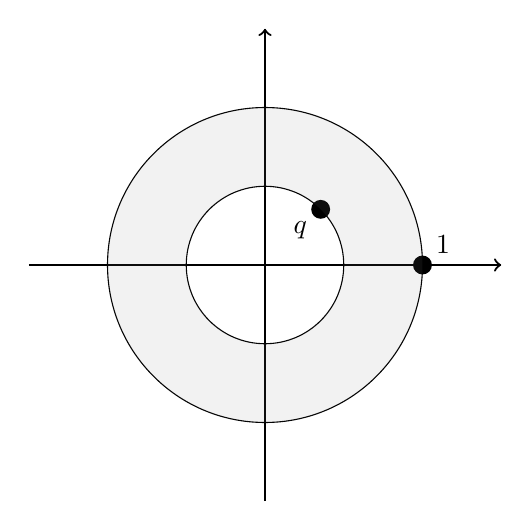
\begin{tikzpicture}[baseline=(current bounding box.center)]
% http://tex.stackexchange.com/questions/202607/drawing-discs-with-circular-holes-with-tikz
    \begin{scope}[thick,font=\scriptsize][set layers]
    \draw [->] (-3,0) -- (3,0);
    \draw [->] (0,-3) -- (0,3);
    \end{scope}
    \draw[solid] (0,0) circle (1);
    \draw[solid] (0,0) circle (2);
    \fill (2,0) circle (0.12) ++(0.26,0.26) node {$1$};
    \fill (0.707,0.707) circle (0.12) ++(-0.26,-0.26) node {$q$};
    \path [draw=none, fill=gray, even odd rule, fill opacity = 0.1] (0,0) circle (2) (0,0) circle (1);
\end{tikzpicture}
\quad \quad $\rightsquigarrow$ \quad \quad
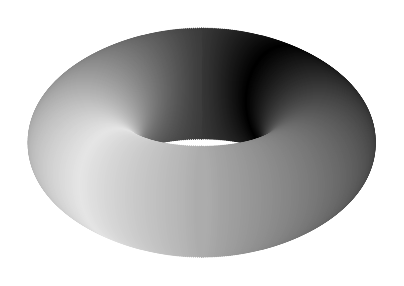
\begin{tikzpicture}[baseline=(current bounding box.center)]
% http://www.texample.net/tikz/examples/smooth-maps/
    \foreach \x in {90,89,...,-90} { % change 89 to 80 or 45 for speed
    % \elrad is the x-radius of the ellipse (technically, a circle seen
    % from side on at angle \x).  The 'max' is because at small angles
    % then the real ellipse is too thin and the torus doesn't ``fill
    % out'' nicely.
    \pgfmathsetmacro\elrad{20*max(cos(\x),.1)}
    % We draw the torus from the back to the front to get the right
    % layering effect.  To tint it, we define colours according to the
    % angle, but need different colours for the left and right pieces.
    % It'd be nice if the xcolor colour specification could take something
    % computed by pdfmath, such as {red!\tint} but it doesn't appear to
    % work, so we define the colours explicitly.
    \pgfmathsetmacro\ltint{.9*abs(\x-45)/180}
    \pgfmathsetmacro\rtint{.9*(1-abs(\x+45)/180)}
    \definecolor{currentcolor}{rgb}{\ltint, \ltint, \ltint}
    % This draws the right-hand circle.
    \draw[color=currentcolor,fill=currentcolor] 
        (xyz polar cs:angle=\x,y radius=.75,x radius=1.5) 
        ellipse (\elrad pt and 20pt);
    % This sets the colour correctly for the left-hand circle ...
    \definecolor{currentcolor}{rgb}{\rtint, \rtint, \rtint}
    % ... and draws it
    \draw[color=currentcolor,fill=currentcolor] 
        (xyz polar cs:angle=180-\x,radius=.75,x radius=1.5) 
        ellipse (\elrad pt and 20pt);
    % End of foreach statement
    }
\end{tikzpicture}
\end{center}
\caption{Presentation of an elliptic curve as the quotient of an annulus.}\label{AnnulusPicture}
\end{figure}

\begin{definition}
The basic $\theta$--function associated to $E_\Lambda$ is defined by \[\theta_q(u) = \prod_{m \ge 1} (1 - q^m) (1 + q^{m-\frac{1}{2}}u) (1 + q^{m-\frac{1}{2}}u^{-1}) = \sum_{n \in \Z} u^n q^{\frac{1}{2} n^2}.\]  Given two rational numbers $0 \le a, b \le 1$, we can also shift the zero-set of $\theta_q$ in the $1$ and $q$ directions by the fractions $a$ and $b$, giving translated $\theta$--functions: \[\theta_q^{a,b}(u) = \left(q^{\frac{a^2}{2}} \cdot u^a \cdot \exp(2 \pi i a b) \right) \cdot \theta_q(u q^a \exp(2 \pi i b)).\]
\end{definition}

The basic $\theta$--function vanishes on the set $\{\exp(2 \pi i (\frac{1}{2}m + \frac{\tau}{2}n))\}$, i.e., at the center of the fundamental annulus.  Since it has no poles, it cannot descend to give a function on $\C^\times / q^{\Z}$, and its failure to descend is witnessed by its imperfect periodicity relation: \[\theta_q(qu) = u^{-1} q^{\frac{-1}{2}} \theta_q(u).\]

\begin{lemma}[{\cite[Proposition 10.2.6]{Husemoller}}]
For any $N > 0$, define $V_q[N]$ to be the space of functions $f\co \C^\times \to \C$ satisfying \[f(q u) = u^{-N}  q^{-N^2/2} f(u).\]  Then, $V_q[N]$ has $\C$--dimension $N^2$, and the functions $\theta_q^{a, b}$ give a basis as $a$ and $b$ range over rational numbers with denominator $N$. \qed
\end{lemma}

Even though these functions do not themselves descend to $\C^\times / q^{\Z}$, we can collectively use them to construct a map to complex projective space, where the quasi-periodicity relations will mutually cancel in homogeneous coordinates.
\begin{theorem}[{\cite[Proposition 10.3.2]{Husemoller}}]
Consider the map
\begin{align*}
\C / (N \cdot \Lambda) & \xrightarrow{f_{(N)}} \P^{N^2-1}(\C), \\
z & \mapsto [\cdots : \theta_q^{i/N, j/N}(z) : \cdots].
\end{align*}
For $N > 1$, this map is an embedding. \qed
\end{theorem}

\begin{example}
Let us expand this in the case of $N = 2$.  The four functions involved are labeled $\theta_q^{0,0}$, $\theta_q^{0,1/2}$, $\theta_q^{1/2,0}$, and $\theta_q^{1/2,1/2}$, and we record their zero loci in \Cref{ThetaFunctionsTable}.  The image of $f_{(2)}$ in $\P^{2^2 - 1}(\C)$ is cut out by the equations
\begin{align*}
A^2 x_0^2 & = B^2 x_1^2 + C^2 x_2^2, &
A^2 x_3^2 & = C^2 x_1^2 - B^2 x_2^2,
\end{align*}
where
\begin{align*}
x_0 & = \theta_q^{0, 0}(u^2), &
x_1 & = \theta_q^{0, 1/2}(u^2), &
x_2 & = \theta_q^{1/2, 0}(u^2), &
x_3 & = \theta_q^{1/2, 1/2}(u^2)
\end{align*}
and
\begin{align*}
A & = \theta_q^{0, 0}(0) = \sum_n q^{n^2}, &
B & = \theta_q^{0, 1/2}(0) = \sum_n (-1)^n q^{n^2}, &
C & = \theta_q^{1/2, 0}(0) = \sum_n q^{(n + 1/2)^2},
\end{align*}
upon which there is the additional ``Jacobi'' relation \[A^4 = B^4 + C^4.\]
\end{example}

\begin{figure}
\begin{center}
\begin{tabular}{@{}cc@{}} \toprule
Function & Zero locus \\
\midrule
$\theta_q^{0,0}$ & $q^{\Z} \cdot q^{1/2} \cdot i$ \\
$\theta_q^{0,1/2}$ & $q^{\Z} \cdot q^{1/2}$ \\
$\theta_q^{1/2,0}$ & $q^{\Z} \cdot i$ \\
$\theta_q^{1/2,1/2}$ & $q^{\Z}$. \\ \bottomrule
\end{tabular}
\end{center}
\caption{Standard $\theta$--functions and their offsets}\label{ThetaFunctionsTable}
\end{figure}

\begin{remark}
This embedding of $E_\Lambda$ as an intersection of quadric surfaces in $\CP^3$ is quite different from the Weierstrass embedding.  Nonetheless, the embeddings are analytically related.  Namely, there is an equality \[\frac{d^2}{dz^2} \log \theta_q(u) = \wp_\Lambda(z).\]  Separately, Weierstrass considered a function $\sigma_\Lambda$, defined by \[\sigma_\Lambda(z) = z \prod_{\omega \in \Lambda \setminus 0} \left( 1 - \frac{z}{\omega} \right) \cdot \exp \left[ \frac{z}{\omega} + \frac{1}{2} \left( \frac{z}{\omega} \right)^2 \right],\] which also has the property that its second logarithmic derivative is $\wp$ and so is ``basically $\theta_q^{1/2,1/2}$''.  In fact, any elliptic function can be written in the form \[c \cdot \prod_{i=1}^n \frac{\sigma_\Lambda(z - a_i)}{\sigma_\Lambda(z - b_i)}.\]
\end{remark}

The $\theta$--functions version of the story has two main successes: it continues to make sense in algebraic geometry, without invoking transcendental functions, and in fact there is a version of this story for an \emph{arbitrary} abelian variety.  It turns out that all abelian varieties are projective, and the theorem sitting at the heart of this claim is
\begin{corollary}[{``Theorem of the Cube'', \cite[Corollary I.6.4 and Theorem I.7.1]{Milne}}]\label{Theta3IsTrivial}
Let $A$ be an abelian variety, let $p_i: A \times A \times A \to A$ be the projection onto the $i${\th} factor, and let $p_{ij} = p_i +_A p_j$, $p_{ijk} = p_i +_A p_j +_A p_k$.  Then for any invertible sheaf $\L$ on $A$, the sheaf \[\Theta^3(\L) := \frac{p_{123}^* \L \otimes p_1^* \L \otimes p_2^* \L \otimes p_3^* \L}{p_{12}^* \L \otimes p_{23}^* \L \otimes p_{31}^* \L \otimes p_\emptyset^* \L} = \bigotimes_{I \subseteq \{1, 2, 3\}} (p_I^* \L)^{(-1)^{|I| - 1}}\] on $A \times A \times A$ is trivial.  If $\L$ is rigid (i.e., it has a specified trivialization at the identity point of $A$), then $\Theta^3(\L)$ is \emph{canonically} trivialized by a section $s(A; \L)$. \qed
\end{corollary}

\begin{remark}
One way to read the Theorem of the Cube is that a weight zero divisor on an abelian variety is principal (i.e., it is the zeroes and poles of a meromorphic function) if and only if its nodes sum to zero.  The meromorphic function you construct this way is unique up to scale, so if you impose a normalization condition at the identity point, you get a unique such function.  Altogether, this gives a pairing between $(A \times A)^*$ and $A$, which can be reconsidered as a multiplication map $A \times A \to A$.
\end{remark}

\begin{remark}
The section $s(A; \L)$ satisfies three familiar properties:
\begin{itemize}
\item It is symmetric: pulling back $\Theta^3 \L$ along a shuffle automorphism of $A^3$ yields $\Theta^3 \L$ again, and the pullback of the section $s(A; \L)$ along this shuffle agrees with the original $s(A; \L)$ across this identification.
\item It is rigid: by restricting to $* \times A \times A$, the tensor factors in $\Theta^3 \L$ cancel out to give the trivial bundle over $A \times A$.  The restriction of the section $s(A; \L)$ to this pullback bundle agrees with the extension of the rigidifying section.
\item It satisfies a $2$--cocycle condition: in general, we define \[\Theta^k \L := \bigotimes_{I \subseteq \{1, \ldots, k\}} (p_I^* \L)^{(-1)^{|I| - 1}}.\]  In fact, $\Theta^{k+1} \L$ can be written as a pullback of $\Theta^k \L$: \[\Theta^{k+1} \L = \frac{(p_{12} \times \id_{A^{k-1}})^* \L}{(p_1 \times \id_{A^{k-1}})^* \L \otimes (p_2 \times \id_{A^{k-1}})^* \L},\] and pulling back a section $s$ along this map gives a new section \[(\delta s)(x_0, x_1, \ldots, x_k) := \frac{s(x_0 +_A x_1, x_2, \ldots, x_k)}{s(x_0, x_2, \ldots, x_k) \cdot s(x_1, x_2, \ldots, x_k)}.\]  Performing this operation on the first and second factors yields the defining equation of a $2$--cocycle.
\end{itemize}
\end{remark}

\begin{remark}
The proof of projectivity arising from this method rests on choosing a line bundle on $A$, extracting from it a very ample line bundle, and then constructing some generating global sections to get an embedding into $\P(\L^{\oplus n})$~\cite[Remark II.7.8.2]{Hartshorne}.  Mumford~\cite{MumfordEquationsI} showed that a choice of ``$\theta$--structure'' on $(A, \L)$, which is only slightly more data, gives a canonical choice of generating global sections as well as a canonical identification of $\P(\L^{\oplus n})$ with a \emph{fixed} projective space.  This is suitable for studying how these equations change as one considers different points in the moduli of abelian varieties~\cite{MumfordEquationsII,MumfordEquationsIII}.
\end{remark}

\begin{remark}[{\cite[Section 4]{Breen}}]
Breen presented a relative version of this story that applies to arbitrary \emph{commutative group schemes}, where the basic objects are a choice of line bundle $\L$ over a commutative group scheme $A$, a choice of trivialization of $\Theta^3 \L$, and an epimorphism $\pi\co A' \to A$ that trivializes $\L$.
\end{remark}

Finally, we remark that the function \[e\co C^3(\G; \Gm) \to \InternalHom{FormalGroups}(\G_a^{\sm 2}, \G_m)\] considered in \Cref{ChromaticKUCoopnsSection} also manifests in the theory of abelian varieties.  Let $A$ be an abelian variety equipped with a line bundle $\L$.  Suppose that $s$ is a symmetric, rigid section of $\Theta^3 \L$, sometimes called a \textit{cubical structure on $\L$}.  Using the identification $(p_{12} - p_1 - p_2)^* \Theta^2 \L = \Theta^3 \L$, this induces the structure of a \textit{symmetric biextension} on $\Theta^2 \L$ via the multiplication maps
\begin{align*}
(\Theta^2 \L)_{x, y} \otimes (\Theta^2 \L)_{x', y} & \to (\Theta^2 \L)_{x + x', y}, &
(\Theta^2 \L)_{x, y} \otimes (\Theta^2 \L)_{x, y'} & \to (\Theta^2 \L)_{x, y + y'}.
\end{align*}

\begin{definition}
There is a canonical piece of gluing data on this biextension, in the form of an isomorphism of pullback bundles
\begin{align*}
e_{p^j}\co (p^j \times 1)^* \L|_{A[p^j] \times A[p^j]} & \cong (1 \times p^j)^* \L|_{A[p^j] \times A[p^j]}, \\
(\ell, x, y) & \mapsto \left(\ell \cdot \prod_{k=1}^{p^j-1} \frac{s(x, [k]x, y)}{s(x, [k]y, y)} \right).
\end{align*}
This function $e_{p^j}$ is called the \textit{($p^j$){\th} Weil pairing}.
\end{definition}

\begin{figure}
\begin{center}
\begin{tikzpicture}[x  = {(-0.707cm,-0.707cm)},
                    y  = {(0.9659cm,-0.25882cm)},
                    z  = {(0cm,1cm)},
                    scale = 1.8,
                    color = {lightgray}]
% style of faces
\tikzset{facestyle/.style={fill=black!25,draw=black,very thin,line join=round,opacity=.4},slicestyle/.style={fill=black!25,draw=black,very thin,line join=round,opacity=.8}}
%\tikzset{facestyle/.style={fill=cyan,draw=blue,very thin,line join=round,opacity=.4},slicestyle/.style={fill=cyan,draw=blue,very thin,line join=round,opacity=.7}}
% face "back" 
\begin{scope}[canvas is zy plane at x=0]
  \path[facestyle,shade] (0,0) rectangle (2,2);
\end{scope}
% face  "left"
\begin{scope}[canvas is zx plane at y=0]
  \path[facestyle,shade] (0,0) rectangle (2,2);
\end{scope}
% face "down"
\begin{scope}[canvas is yx plane at z=0]
  \path[facestyle,color=lightgray] (0,0) rectangle (2,2);
\end{scope}
% face "red slice back"
\begin{scope}[canvas is zy plane at x=1.5]
  \path[slicestyle,color=black!50] (0,0) rectangle (2,0.5);
\end{scope}
% face "green slice back"
\begin{scope}[canvas is zx plane at y=0.5]
  \path[slicestyle,color=black] (0,0) rectangle (2,1.5);
\end{scope}
% face "red slice front"
\begin{scope}[canvas is zy plane at x=1.5]
  \path[slicestyle,color=black!50] (0,0.5) rectangle (2,2);
\end{scope}
% face "green slice front"
\begin{scope}[canvas is zx plane at y=0.5]
  \path[slicestyle,color=black] (0,1.5) rectangle (2,2);
\end{scope}
% face "front"
\begin{scope}[canvas is zy plane at x=2]
  \path[facestyle] (0,0) rectangle (2,2);
\end{scope}
% face  "right"
\begin{scope}[canvas is zx plane at y=2]
  \path[facestyle] (0,0) rectangle (2,2);
\end{scope}
% face "up" 
\begin{scope}[canvas is yx plane at z=2]
  \path[facestyle] (0,0) rectangle (2,2);
\end{scope}
% labels
\draw[very thin,black,line join=round]
     (2,0,0) -- node [below,black] {$A$} (2,2,0);
\draw[very thin,black,line join=round]
     (2,2,0) -- node [right,black] {$A$} (0,2,0);
\draw[very thin,black,line join=round]
     (0,2,0) -- node [right,black] {$\Gm$} (0,2,2);
\draw[very thin,black,line join=round]
     (2,0.5,0) -- node [below,black] {$a_1$} (2,0.5,0);
\draw[very thin,black,line join=round]
     (1.5,2,0) -- node [right,black] {$a_2$} (1.5,2,0);
\end{tikzpicture}
\hspace{0.5em}
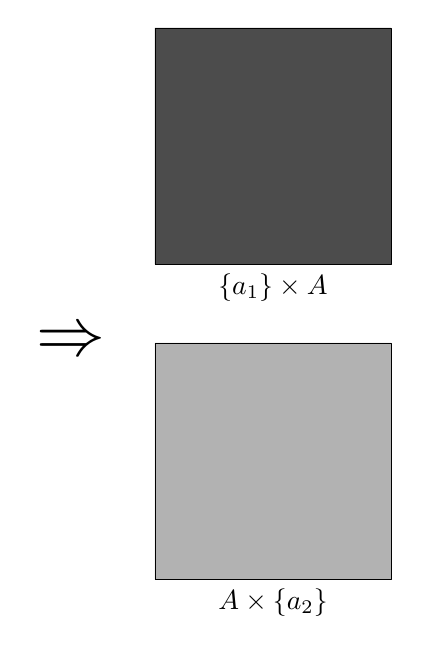
\begin{tikzpicture}
    \draw[very thin,black,line join=round,fill=black!30]
        (0,1) -- node [below,black] {$A \times \{a_2\}$} (3,1) -- node[right,black] {$\Gm$} (3,4) -- (0,4) -- (0,1);
    \draw[very thin,black,line join=round,fill=black!70]
        (0,5) -- node [below,black] {$\{a_1\} \times A$} (3,5) -- node[right,black] {$\Gm$} (3,8) -- (0,8) -- (0,5);
    \node[anchor=east] at (-0.5,4) {\Huge $\Rightarrow$};
\end{tikzpicture}
\end{center}
\caption{Extensions contained in a biextension.}
\end{figure}

\begin{remark}
In the case that $A$ is an elliptic curve, this agrees with the usual definition of its ``Weil pairing''.  In the case of a \emph{complex} elliptic curve $\C / (1, \tau)$, this degenerates further to the assignment \[\left( \frac{a}{n}, \frac{b}{n} \tau \right) \mapsto \exp\left(-2\pi i \frac{ab}{n}\right).\]
\end{remark}

We now actually leverage this arithmetic geometry by placing ourselves in a situation where algebraic topology is directly linked to abelian varieties.

\begin{definition}\label{DefnEllipticSpectrum}
An \textit{elliptic spectrum} consists of a even--periodic ring spectrum $E$, a (generalized) elliptic curve $C$ over $\Spec E_0$, and a fixed isomorphism \[\phi\co C^\wedge_0 \xrightarrow{\cong} \CP^\infty_E.\]  A map among such spectra consists of a map of ring spectra $f\co E \to E'$ together with a specified isomorphism of elliptic curves $\psi\co f^* C \to C'$.\footnote{Elliptic curves and cohomology theories can be brought much closer together still, as in Lurie's framework~\cite[Sections 4 and 5.3]{LurieSurveyOfEll}.}
\end{definition}

\begin{remark}
Our preference for \emph{isomorphisms} of elliptic curves rather than general homomorphisms is prompted by our study of stable operations: we have seen that a stable operation between complex-oriented ring spectra can only ever give rise to an isomorphism of formal group laws (incorporating a suitable base change).  More broadly, we have also found that the collection of possible isomorphisms of formal group laws organizes into the \textit{stable context}, a very important object in our study.  In the next Case Study, we will develop a theory (with an attendant notion of context) which incorporates \emph{isogenies} of elliptic curves in addition to isomorphisms.
\end{remark}

Coupling \Cref{DefnEllipticSpectrum} to \Cref{BU6Triumvirate} and \Cref{Theta3IsTrivial}, we conclude the following:
\begin{corollary}\label{EllipticSpectraAreOriented}
An elliptic spectrum $(E, C, \phi)$ receives a canonical map of ring spectra \[MU[6, \infty) \to E.\]  This map is natural in choice of elliptic spectrum: if $(E, C, \phi) \to (E', C', \phi')$ is a map of elliptic spectra, then the triangle
\begin{center}
\begin{tikzcd}
& MU[6, \infty) \arrow{ld} \arrow{rd} \\
E \arrow{rr} & & E'
\end{tikzcd}
\end{center}
commutes. \qed
\end{corollary}

\begin{example}
Our basic example of an elliptic curve was $E_\Lambda = \C / \Lambda$, with $\Lambda$ a complex lattice.  The projection $\C \to \C / \Lambda$ has a local inverse which defines an isomorphism of formal groups \[\phi\co (E_\Lambda)^\wedge_0 \xrightarrow{\cong} \G_a \times \Spec \C,\] as well as an isomorphism of cotangent spaces
\begin{center}
\begin{tikzcd}
T^0 (E_\Lambda)^\wedge_0 \arrow[iso]{r} \arrow[iso, leftarrow]{d} & \C \arrow[equal]{d} \\
T^0 (\G_a \times \Spec \C) \arrow[iso]{r} & \C.
\end{tikzcd}
\end{center}
Accordingly, we define an elliptic spectrum $HE_\Lambda P$ whose underlying ring spectrum is $H\C P$ and whose associated elliptic curve and isomorphism are $E_\Lambda$ and $\phi$.  This spectrum receives a natural map \[MU[6, \infty) \to HE_\Lambda P,\] which to a bordism class $M \in MU[6, \infty)_{2n}$ assigns an element $\Phi_\Lambda(M) \cdot u_\Lambda^n \in HE_\Lambda P_{2n}$, where $u_\Lambda$ is the canonical section of $\widetilde{\pi_2 HE_\Lambda P} = \omega_{\CP^\infty_{HE_\Lambda P}}$ and $\Phi_\Lambda(M) \in \C$ is some resulting complex number.
\end{example}

\begin{example}
The naturality of the $MU[6, \infty)$--orientation moves us to consider more than one elliptic spectrum at a time.  If $\Lambda'$ is another lattice with $\Lambda' = \lambda \cdot \Lambda$, then the multiplication map $\lambda\co \C \to \C$ descends to an isomorphism $E_\Lambda \to E_{\Lambda'}$ and hence a map of elliptic spectra $HE_{\Lambda'}P \to HE_\Lambda P$ acting by $u_{\Lambda'} \mapsto \lambda u_\Lambda$.  The commuting triangle in \Cref{EllipticSpectraAreOriented} then begets the \emph{modularity relation} \[\Phi(M; \lambda \cdot \Lambda) = \lambda^{-n} \Phi(M; \Lambda).\]
\end{example}

\begin{example}\label{OrdinaryHomologyInUpperHalfPlaneEx}
This equation leads us to consider all curves $E_\Lambda$ simultaneously---or, equivalently, to consider modular forms.  The lattice $\Lambda$ can be put into a standard form, by picking a basis and scaling it so that one vector lies at $1$ and the other vector lies in the upper half-plane.  This gives a cover \[\h \to \moduli{ell} \times \Spec \C\] which is well-behaved (i.e., unramified) away from the special points $i$ and $e^{2 \pi i / 6}$.  A \textit{complex modular form of weight $n$} is an analytic function $\h \to \C$ which satisfies a certain decay condition and which is quasi-periodic for the action of $SL_2(\Z)$, i.e.,\footnote{That is, for the action of change of basis vectors.} \[f\left(M; \frac{a \tau + b}{c \tau + d} \right) = (c \tau + d)^n f(M; \tau).\]

Using these ideas, we construct a cohomology theory $H \sheaf O_{\h} P$, where $\sheaf O_{\h}$ is the ring of complex-analytic functions on the upper half-plane.  The $\h$--parametrized family of elliptic curves \[\h \times \C / (1, \tau) \to \h,\] together with the logarithm, present $H \sheaf O_{\h} P$ as an elliptic spectrum $H\h P$.  The canonical map $\Phi\co MU[6, \infty) \to H\h P$ specializes at a point to give the functions $\Phi(-; \Lambda)$ considered above, and hence $\Phi(M) \in u^k \cdot \sheaf O_{\h}$ is itself a complex modular form of weight $k$.
\end{example}

In fact, this totalized map $\Phi$ is a ghost of Ochanine and Witten's modular genus from \Cref{OchanineWittenTheorem}, as a bordism class in $MU[6, \infty)_{2n}$ is, in particular, a bordism class in $M\String_{2n}$.  However, they know more about this function than we can presently see: for instance, they claim that it has an integral $q$--expansion.  In terms of the modular form, its $q$--expansion is given by building the Taylor expansion ``at $\infty$'' (using that unspoken decay condition).  In order to use our topological methods, it would be nice to have an elliptic spectrum embodying these $q$--expansions in the same way that $H\h P$ embodied holomorphic functions, together with a comparison map that trades a modular form for its $q$--expansion.  The main ideas leading to such a spectrum come from considering the behavior of $E_\Lambda$ as $\tau$ tends to $i \cdot \infty$.

\begin{definition}
Note that as $\tau$ tends to $i \cdot \infty$, the parameter $q = \exp(2 \pi i \tau)$ tends to $0$.  In the multiplicative model of \Cref{SectionEllipticCurvesAndThetaFunctions}, we considered the punctured complex disk $D'$ with its associated family of elliptic curves \[C'_{\mathrm{an}} = \C^\times \times D' / (u, q) \sim (qu, q).\]  The fiber of $C'$ over a particular point $q \in D'$ is the curve $\C^\times / q^{\Z}$. %  , and $\theta$ determines a holomorphic function on the total space $\C^\times \times D'$.
The Weierstrass equations give an embedding of $C'_{\mathrm{an}}$ into $D' \times \CP^2$ described by \[wy^2 + wxy = x^3 - 5 \alpha_3 w^2 x + -\frac{5 \alpha_3 + 7 \alpha_5}{12}w^3\] for certain functions\todo{Do these have weights?} $\alpha_3$ and $\alpha_5$ of $q$.  At $q = 0$, this curve collapses to the twisted cubic \[wy^2 + wxy = x^3,\] and over the whole open unit disc $D$ we call this extended family $C_{\mathrm{an}}$.

Now let $A \subseteq \Z\ps{q}$ be the subring of power series which converge absolutely on the open unit disk.  It turns out that the coefficients of the Weierstrass cubic (i.e., $5\alpha_3$ and $\frac{1}{12}(5\alpha_3+7\alpha_5)$) lie in $A$, so it determines a generalized elliptic curve $C$ over $\Spec A$, and $C_{\mathrm{an}}$ is the curve given by base-change from $A$ to the ring of holomorphic functions on $D$.\citeme{Find a reference for this. You may be able to look in Morava's Section 5}  The \textit{Tate curve} is the intermediate family $C_{\Tate}$ over the intermediate base $D_{\Tate} = \Spec \Z\ps{q}$, as base-changed from $A$.
\end{definition}

The singular fiber at $q = 0$ prompts us to enlarge our notion of elliptic curve slightly.

\begin{definition}[{\cite[Definitions B.1-2]{AHSTheoremOfTheCube}}]
A \textit{Weierstrass curve} is \emph{any} curve of the form \[C(a_1, a_2, a_3, a_4, a_6) := \left\{ [x : y : w] \in \mathbb P^2 \middle| \begin{array}{c} y^2 w + a_1 xyw + a_3 yw^2 = \\ x^3 + a_2 x^2 w + a_4 x w^2 + a_6 w^3 \end{array} \right\}.\]  A \textit{generalized elliptic curve} over $S$ is a scheme $C$ equipped with maps \[S \xrightarrow{0} C \xrightarrow{\pi} S\] such that $C$ is Zariski--locally isomorphic to a system of Weierstrass curves (in a way preserving $0$ and $\pi$).\footnote{An elliptic curve in the usual sense turns out to be a generalized elliptic curve which is smooth, i.e., the discriminant of the Weierstrass equations is a unit.}\footnote{Unfortunately, ``generalized elliptic curve'' already means something in number theory, but Ando, Hopkins, and Strickland reused this phrase for this definition in their published article.  In a number theorist's language, these are ``stable curves of genus $1$ with specified section in the smooth locus''.  No adjective other than ``generalized'' seems to be much better: singular, for instance, evokes the right idea but is also already taken.}
\end{definition}

\begin{remark}[{\cite[pg.\ 670]{AHSTheoremOfTheCube}}]\label{TwistedCubicGivesGm}
The singularities of a degenerate Weierstrass equation always occur outside of a formal neighborhood of the marked identity point, which in fact still carries the structure of a formal group.  The formal group associated to the twisted cubic is the formal multiplicative group (indeed, the smooth locus of the twisted cubic \emph{is the multiplicative group}), and the isomorphism making the identification extends a family of such isomorphisms $\phi$ over the nonsingular part of the Tate curve.
\end{remark}

\begin{definition}[{\cite[Section 5]{MoravaFormsOfKthy}, \cite[Section 2.7]{AHSTheoremOfTheCube}}]
The generalized elliptic spectrum $K_{\Tate}$, called \textit{Tate $K$--theory}, has as its underlying spectrum $KU\ps{q}$.  The associated generalized elliptic curve is $C_{\Tate}$, and the isomorphism $\CP^\infty_{KU\ps{q}} \cong (C_{\Tate})^\wedge_0$ is $\phi$ from \Cref{TwistedCubicGivesGm}.
\end{definition}

\noindent The trade for the breadth of this definition is that theorems pulled from the study of abelian varities have to be shown to extend uniquely to those generalized elliptic curves which are not smooth curves.

\begin{theorem}[{\cite[Propositions 2.57 and B.25]{AHSTheoremOfTheCube}}]\label{GeneralizedTheta3IsTrivial}
For a generalized elliptic curve $C$, there is a canonical\footnote{Canonical, with a unique continuous extension from the smooth bulk of the moduli of generalized elliptic curves, but \emph{not} actually unique over the singular locus.} trivialization $s$ of $\Theta^3 \sheaf I(0)$ which is compatible with change of base and with isomorphisms.  If $C$ is a smooth elliptic curve, then $s$ agrees with that of \Cref{Theta3IsTrivial}. \qed
\end{theorem}

\begin{corollary}\label{D3thetaTrivializes}
The trivializing section $s$ associated to $C_{\Tate}$ is given by $\delta^{\circ 3} \tilde \theta$, where $\tilde \theta_q$ is a slight modification of the classical $\theta$--function:
\begin{align*}
\tilde \theta_q(u) & = (1 - u)\prod_{n > 0}(1 - q^n u)(1 - q^n u^{-1}), &
\tilde \theta_q(qu) & = -u^{-1} \tilde\theta_q(u).
\end{align*}
\end{corollary}
\begin{proof}
Even though $\tilde \theta$ is not a function on $C_{\Tate}$ because of its quasiperiodicity, it does trivialize both $\pi^* \sheaf I(0)$ for $\pi\co \C^\times \times D \to C_{\Tate}$ and $\sheaf I(0)$ for $(C_{\Tate})^\wedge_0$.  Moreover, the quasiperiodicities in the factors in the formula defining $\delta^3 \tilde \theta|_{(C_{\Tate})^\wedge_0}$ cancel each other out, and the resulting function \emph{does} descend to give a trivialization of $\Theta^3 \sheaf I(0)$.  By the unicity and continuity clauses in \Cref{GeneralizedTheta3IsTrivial}, it must give a formula expressing $s$.
\end{proof}

\begin{definition}
The induced map \[\sigma_{\Tate}\co MU[6, \infty) \to K_{\Tate}\] is called the \textit{complex $\sigma$--orientation}.
\end{definition}

\begin{corollary}\label{WittensTheoremForBU6}
Let $M \in \pi_{2n} MU[6, \infty)$ be a bordism class.  The $q$--expansion of Witten's modular form $\Phi(M)$ has integral coefficients.
\end{corollary}
\begin{proof}
The span of elliptic spectra equipped with $MU[6, \infty)$--orientations
\begin{center}
\begin{tikzcd}
& MU[6, \infty) \arrow["\Phi"]{rd} \arrow{d} \arrow["\sigma_{\Tate}"']{ld} \\
K_{\Tate} \arrow{r} & K_{\Tate} \otimes \C & H\h P \arrow{l}
\end{tikzcd}
\end{center}
models $q$--expansion.  The arrow $K_{\Tate} \to K_{\Tate} \otimes \C$ is injective on homotopy, which shows that the $q$--expansion of $\Phi(M)$ lands in the subring of integral power series.
\end{proof}

We can use the formula $\sigma_{\Tate} = \delta^3 \tilde \theta$ appearing in \Cref{D3thetaTrivializes} to explicitly understand the genus associated to $\sigma_{\Tate}$ by passing to homotopy groups.  To begin, the appearances of the map $\delta$ in \Cref{BUtoBUZ}, \Cref{BSUToBU}, and \Cref{MSUToMU6} show that $\sigma_{\Tate}$ belongs to the commutative triangle
\begin{center}
\begin{tikzcd}
MU[6, \infty) \arrow["\delta"]{r} \arrow["\sigma_{\Tate}"']{drrr} & MSU \arrow["\delta"]{r} & MU \arrow["\delta"]{r} & MUP \arrow["\tilde \theta"]{d} \\
& & & KU\ps{q}.
\end{tikzcd}
\end{center}
We will analyze this triangle by comparing $\tilde\theta$ to the usual $MUP$--orientation of $KU$, which selects the coordinate $f(u) = 1 - u$ on the formal completion of $\Gm = \Spec \Z[u^\pm]$.  Appealing to \Cref{BUtoBUZ}, the induced $MU$--orientation \[MU \xrightarrow{\delta} MUP \xrightarrow{\Td} KU\] sends $f$ to the rigid section $\delta f$ of \[\Theta^1 \sheaf I(0) = \sheaf I(0)_0 \otimes \sheaf I(0)^{-1} \cong \omega \otimes \sheaf I(0)\] given by \[\delta f = \frac{1}{1 - u} \left( - \frac{du}{u} \right).\]  The difference between $\delta \Td$ and $\delta \tilde\theta$ is expressed by an element $\psi \in C^1(\widehat C_{\Tate}; \Gm)$, given explicitly by the quotient formula \[\psi = \left(\frac{\Td(1)}{\Td(u)}\right)^{-1} \cdot \frac{\tilde \theta_q(1)}{\tilde \theta_q(u)} = \prod_{n \ge 1} \frac{(1 - q^n)^2}{(1 - q^n u)(1 - q^n u^{-1})}.\]  This gives a re-expression of $\delta \tilde\theta$ as the composite \[\delta \tilde\theta\co MU \xrightarrow{\eta_R} MU \sm MU \simeq MU \sm BU_+ \xrightarrow{\delta\Td \sm \psi} K_{\Tate},\] and hence its effect on a line bundle is determined by the evaluation of this characteristic series: \[\psi(1 - \L) = \prod_{n \ge 1} \frac{(1 - q^n)^2}{(1 - q^n \L)(1 - q^n \L^{-1})}.\]  Its effect on vector bundles in general is determined by the splitting principle and an exponential law, which after some computation\citeme{AHS} gives the generic formula \[\psi(\dim V \cdot 1 - V) = \bigotimes_{n \ge 1} \bigoplus_{j \ge 0} \Sym^j(\dim V \cdot 1 - V \otimes_{\R} \C) q^{jn} =: \bigotimes_{n \ge 1} \Sym_{q^n}(- \bar V_{\C}).\]  Finally, the map $(\eta_R)_*\co MU_* \to \pi_*(MU \sm \Susp^\infty_+ BU)$ sends a manifold $M$ with stable normal bundle $\nu$ to the pair $(M, \nu)$, so we at last compute
\begin{align*}
\sigma_{\Tate}(M \in \pi_{2n} MU[6, \infty)) & = (\delta \Td \sm \theta')(M, \nu) \\
& =: \Td\left(M; \bigotimes_{n \ge 1} \Sym_{q^n}(\bar \tau_{\C}) \right).
\end{align*}
This is exactly Witten's formula for his genus, as applied to complex manifolds with first two Chern classes trivialized.

\begin{remark}[{\cite[Section 1.5]{RezkFelixKlein}}]
Witten defines his characteristic series for \emph{oriented} manifolds by the formula
\begin{align*}
K_{\mathrm{Witten}}(x) & = \exp\left( \sum_{k=2}^\infty 2 G_{2k}(\tau) \cdot \frac{x^{2k}}{(2k)!} \right) \\
& = \frac{x/2}{\sinh(x/2)} \cdot \left(\prod_{n=1}^\infty \frac{(1 - q^n)^2}{(1 - q^n u)(1 - q^n u^{-1})}\right) \cdot e^{-G_2(\tau) x^2},
\end{align*}
where $G_{2k}$ is the $2k${\th} Eisenstein series.  Noting that $G_2$ is \emph{not} a modular form, the condition that $p_1(M) / 2$ vanish is precisely the condition that $G_2$ contribute nothing to the sum, so that the remainder \emph{is} a modular form.
\end{remark}

\begin{remark}[{\cite{AndoMorava}}]
Another location where this series $\psi$ appears is in the theory of Tate $p$--divisible groups of Ando and Morava (and, in some sense, in the sense of Katz and Mazur).  For a formal group $\G$ over $\Spf R$ with group law $+_\phi$, they consider the Weierstrass product \[\Theta_{\phi}(x; q) = x \cdot \prod_{\substack{k \in \Z \\ k \ne 0}} \frac{(x +_\phi [k]_\phi(q))}{[k]_\phi(q)} \in R\ps{x,q},\] which plays the role of a kind of $\theta$--function for $\G$.  They also connect this series the quotient function mapping to the group scheme $\G / q^{\Z}$ (in the sense of \todo{CITE ME OUT OF CHAPTER 6}), which they further identify as the universal extension of $\G$ by a constant $p$--divisible group of dimension $1$.  In the presense of a global object $\mathbb G$ specializing to $\G$ (as in the case of $\G_a$ or $\G_m$), they show how to modify this product to an analytically convergent power series, recovering the characteristic series for the $\widehat A$--genus and the $L$--genus.  The higher height analogues of these results seem very mysterious and very interesting.\footnote{Morava is generally full of interesting ideas about genera---see, for instance,~\cite{MoravaMotivicThomIso}.}
\end{remark}

\begin{remark}[{\cite{AFG}}]
Ando, French, and Ganter have given a construction that convert $MU[2k, \infty)$--orientations of a spectrum $E$ to $MU[2(k-1), \infty)$--orientations of the pro-spectrum $E^{\CP^\infty_{-\infty}}$.  Performing this operation to the $\sigma$--orientation of $K^{\Tate}$ gives the ``two--variable Jacobi genus'', which assigns $SU$--manifolds to certain classes in $\pi_0 (K^{\Tate})^{\CP^\infty_{-\infty}} = \Z\ps{q}(\!(y)\!)$ connected to meromorphic Jacobi forms.
\end{remark}













\section{Chromatic \texorpdfstring{$\Spin$}{Spin} and \texorpdfstring{$\String$}{String} orientations}

We now turn to understanding $M\String$--orientations in turns of $MU[6, \infty)$--orientations.  We will approach this in successive passes, keeping the desired picture sharp the entire time but introducing generality slowly.  Unfortunately, most of the original source material~\cite{HAS,StricklandFSKS} for this has not been published, and hence it is difficult to give references.\footnote{Versions of some of this have appeared in work of Kitchloo and Laures~\cite{KitchlooLaures}.}  We have gone to some lengths to prepare the reader for the sorts of arguments that appear here: they are not so different from the arguments appearing elsewhere in this chapter.

We begin at the maximally simple situation, where $2$ is inverted.  In this case, the Wood cofiber sequence \[\Susp kO \xrightarrow{\eta} kO \xrightarrow{c} kU \xrightarrow{\lambda} \Susp^2 kO\] becomes split, since $\eta$ is a $2$--torsion element.  By considering different underlying infinite-loopspaces, this gives a number of identifications:
\begin{center}
\begin{tikzcd}[row sep=0em]
\OS{(-)}{0}: & BO \times \Z \arrow{r} & BU \times \Z \arrow{r} & \OS{kO}{2}, \\
\OS{(-)}{2}: & \OS{kO}{2} \arrow{r} & BU \arrow{r} & \OS{kO}{4}, \\
\OS{(-)}{4}: & \OS{kO}{4} \arrow{r} & BSU \arrow{r} & \OS{kO}{6}, \\
\OS{(-)}{6}: & \OS{kO}{6} \arrow{r} & BU[6, \infty) \arrow{r} & B\String.
\end{tikzcd}
\end{center}
Next, by recognizing $c\co kO \to kU$ as the complexification map, we note that it lies in fixed points for complex-conjugation on $kU$.  The other gain that inverting $2$ gets us is an idempotent selecting this fixed point subspectrum: there are a pair of orthogonal idempotents
\begin{align*}
P_+ & = \frac{1 + \xi}{2}, &
P_- & = \frac{1 - \xi}{2},
\end{align*}
which reidentify the splitting $kU \simeq kO \vee \Susp^2 kO$ in various equivalent ways: \[kU \simeq kO \vee \Susp^2 kO \simeq \im P_- \vee \im P_+ \simeq \ker P_+ \vee \ker P_- \simeq \left( \frac{kU}{\im P_+} \right) \vee \left( \frac{kU}{\im P_-} \right).\]  This last identification immediately gives access to the following result:
\begin{lemma}
For $E$ a complex-orientable ring spectrum with $1/2 \in \pi_0 E$, we have
\begin{align*}
B\String_E & = C_3(\CP^\infty_E) / ([a, b, c] = -[-a, -b, -c]), \\
\Spec E_0 B\String & = \left\{ f \in C^3(\CP^\infty_E; \Gm) \middle| f(a, b, c) = \frac{1}{f(-a, -b, -c)} \right\} \subseteq C^3(\CP^\infty_E; \Gm).
\end{align*}
\end{lemma}
\begin{proof}[Proof sketch]
This is a matter of translating the splittings above across \Cref{BU6Triumvirate}.  The complex-conjugation map $\xi$ acts on $C_k(\G)$ according to \[\xi[a_1, \ldots, a_n] = (-1)^n [-a_1, \ldots, -a_n],\] which encodes $B\String_E$ as the quotient of $BU[6, \infty)_E$ by $\im P_-$.  Finally, the claim about the homological scheme follows from the description of the cohomological formal scheme by Cartier duality.
\end{proof}

The repeated appearances of the terms in the above splittings suggest that the composite \[\tau\co kU \xrightarrow{\lambda} \Susp^2 kO \xrightarrow{\Susp^2 c} \Susp^2 kU\] of the maps in two adjacent cofiber sequences itself plays an interesting role.  This is the map that encodes surjecting onto one factor in the preceding splitting, then reincluding it into the next splitting.
\begin{lemma}
At the level of formal schemes, the map $\tau$ acts by
\begin{align*}
\tau\co C_k(\G) & \to C_{k+1}(\G) \\
[a_1, \ldots, a_k] & \mapsto [a_1, \ldots, a_k, -(a_1 + \cdots + a_k)].
\end{align*}
\end{lemma}
\begin{proof}
We are in pursuit of the following calculation in $kU^* (\CP^\infty)^{\times (k+1)}$ encoding complexification after decomplexification:
\begin{align*}
\beta^k x_1 \cdots x_k + \beta^k \overline{x_1} \cdots \overline{x_k} & = (1 - \L_1) \cdots (1 - \L_k) + (1 - \overline \L_1) \cdots (1 - \overline \L_k) \\
& = (1 - \L_1) \cdots (1 - \L_k) + \overline \L_1 \cdots \overline \L_k (\L_1 - 1) \cdots (\L_k - 1) \\
& = (1 - \L_1) \cdots (1 - \L_k) (1 - (-1)^{k+1} \overline \L_1 \cdots \overline \L_k) \\
& = \beta^{k+1} x_1 \cdots x_k \cdot \xi^* \mu^*(x_1, \ldots, x_k). \qedhere
\end{align*}
\end{proof}
Still in the case where $E$ is local away from $2$, we can use this alternative description of the inclusion of the $P_-$ factor to deduce an alternative description of the formal scheme associated to $B\String$:
\begin{corollary}
For $E$ a complex-orientable ring spectrum with $1/2 \in \pi_0 E$, we have
\begin{align*}
B\String_E & = C_3(\CP^\infty_E) / ([a, b, -a-b] = 0), \\
\Spec E_0 B\String & = \left\{ f \in C^3(\CP^\infty_E; \Gm) \middle| f(a, b, -a-b) = 1 \right\} \subseteq C^3(\CP^\infty_E; \Gm). \qed
\end{align*}
\end{corollary}

\begin{definition}
We denote this last functor by $\Sigma^3(\CP^\infty_E; \Gm)$, and more generally if $\L$ is a line bundle on $\CP^\infty_E$ then $\Sigma^3(\CP^\infty_E; \L)$ will denote the subscheme of $C^3(\CP^\infty_E; \L)$ of those trivializations which restrict to the rigidifying trivialization of $\Theta^3 \L$ on the subscheme of $(\CP^\infty)^{\times 3}$ specified by $[a, b, -a-b]$.  Such trivializations are referred to as \textit{$\Sigma$--structures on $\L$}, following Breen~\cite[Section 5]{Breen}.
\end{definition}

\begin{corollary}\label{OddPrimaryMStringTriumvirate}
For $E$ a complex-orientable ring spectrum with $1/2 \in \pi_0 E$, the functor $\Sigma^3(\CP^\infty_E; \sheaf I(0))$ is isomorphic to the affine scheme $\Spec E_0 M\String$.  Moreover, the $E_0$--points of this scheme biject with ring spectrum maps $M\String \to E$. \qed
\end{corollary}

\begin{remark}
One of the most pleasant features of the case where $2$ is inverted is that real orientations can not only be identified, but the projection idempotents mean that they can be \emph{crafted} from complex orientations, and the idempotents have a recognizable effect on the traditional mechanisms for specifying orientations.  For instance, the Conner--Floyd orientation on $K$--theory is specified by the classical logarithm, and the associated real orientation formed by projection to the positive idempotent has logarithm \[\operatorname{tanh}^{-1}(x) = \frac{-\ln(1 - x) + \ln(1 + x)}{2},\] i.e., the average of the logarithm and its conjugate.  The resulting orientation is commonly referred to as the \textit{Atiyah--Bott--Shapiro orientation}, whose associated genus is the \textit{$\widehat A$--genus}.  Similar techniques give access to connective real orientations associated to preexisting connective complex orientations.
\citeme{Ahat genus?}
\end{remark}

We now turn to the \emph{much} more complicated setting where $2$ is not invertible, where we again aim to identify $M\String$--orientations of a complex-orientable cohomology theory with certain $\Sigma$--structures.  This is not possible in much generality, a situation which is hinted by the analogous lower-order case: complex-orientability is flatly \emph{not enough} to conclude anything about whether a cohomology theory admits an $MO$--orientation, which we saw in \Cref{MOSplitsIntoHF2s} to be actually equivalent to admitting an $\HFtwo$--algebra structure.  In order to get a handle on the task in front of us, consider the following diagram of fiber sequences of infinite loopspaces:
\begin{center}
\begin{tikzcd}[column sep=0em]
& \Spin / SU \arrow[equal]{ld} \arrow{rr} \arrow[equal]{dd} & & BU[6, \infty) \arrow[equal]{ld} \arrow{rr} \arrow{dd} & & B\String \arrow[equal]{ld} \arrow{dd} \\
\OS{kO[8, \infty)}{-2} \arrow[crossing over]{rr} & & \OS{kU[8, \infty)}{-2} \arrow[crossing over]{rr} & & \OS{(\Susp^2 kO)[8, \infty)}{-2} \\
& \Spin/SU \arrow[equal]{ld} \arrow{rr} & & BSU \arrow[equal]{ld} \arrow{rr} & & B\Spin \arrow[equal]{ld} \\
\OS{kO[6, \infty)}{-2} \arrow{rr} \arrow[equal]{uu} & & \OS{kU[6, \infty)}{-2} \arrow{rr} \arrow[leftarrow,crossing over]{uu} & & \OS{(\Susp^2 kO)[6, \infty)}{-2}. \arrow[leftarrow,crossing over]{uu}
\end{tikzcd}
\end{center}
Our program is to analyze the chromatic homology of $\Spin/SU$ as well as the maps to $BU[6, \infty)$ and $BSU$.  We hope to show that the scheme associated to $\Spin/SU$ selects exactly the relations defining $\Sigma$--structures \emph{and} that the map is flat, so that the associated bar spectral sequences
\begin{align*}
\Tor^{E_* \Spin/SU}_{*, *}(E_*, E_* BSU) & \Rightarrow E_* B\Spin, &
\Tor^{E_* \Spin/SU}_{*, *}(E_*, E_* BU[6, \infty)) & \Rightarrow E_* B\String
\end{align*}
collapse to give short exact sequences of Hopf algebras.

We embark on this project with an analysis of the natural bundles classified by the topological objects, so that we can guess the relevant algebraic model.  We have the following complexification and decomplexification maps:
\begin{center}
\begin{tikzcd}
& & \OS{kU}{6} \arrow["\delta"]{d} \\
\OS{kU}{4} \arrow["j"]{r} & \OS{kO}{6} \arrow["\lambda"]{ru} \arrow["i"]{r} & \OS{kU}{4}.
\end{tikzcd}
\end{center}

\begin{lemma}\label{SpinSUComparisonMapIsInj}
Let $E$ be a complex-orientable cohomology theory.  The map $j$ induces an injection \[\Spec E_0(\Spin/SU) \to \Sigma^2(\CP^\infty_E; \Gm).\]
\end{lemma}
\begin{proof}[Proof, with some details omitted]
Recall that our reinterpretation of \Cref{CharacterizationOfBSUUpperE} in \Cref{AdjointBSUExample} passed through the adjoint map $\widehat \Pi_2$ of the natural product bundle $\Pi_2\co (\CP^\infty)^{\times 2} \to BSU$.  We extend the map $\Pi_2$ in two directions: \[\CP^\infty \xrightarrow{(1 - \L)(1 - \overline{\L})} \CP^\infty \times \CP^\infty \xrightarrow{\Pi_2} BSU \xrightarrow{j} \Spin/SU.\]  Checking that this composite is zero on $E$--homology will give a factorization
\begin{center}
\begin{tikzcd}
\Spec E_0 \Spin/SU \arrow["E_0 j"]{r} \arrow[densely dotted]{d} & \Spec E_0 BSU \arrow[equal]{d} \\
\Sigma^2(\CP^\infty_E; \Gm) \arrow{r} & C^2(\CP^\infty_E; \Gm),
\end{tikzcd}
\end{center}
since $\Sigma^2(\CP^\infty_E; \Gm)$ is defined to be the closed subscheme of $C^2(\CP^\infty_E; \Gm)$ of those functions satisfying $f(x, -x) = 1$.

The ordinary homology of $\Spin/SU$ is free and even, so it suffices to check that this map is null in the case $E = H\Z_{(2)}$, since one can then conclude the general case by the Atiyah--Hirzebruch spectral sequence.  Manual calculation in a Serre spectral sequence shows gives the calculation $H\Z_{(2)}{}_*(\Spin/SU) \cong \Gamma_{\Z_{(2)}}[a_{2n+1} \mid n \ge 1]$ as well as that the homological maps induced by $i$ and $j$ are respectively injective and surjective.  In particular, we need only check that the above composite is zero on $H\Z_{(2)}$--homology after postcomposition with $H_*(i)$.  The $SU$--bundle classified by postcomposition with $i$ is \[(1 - \L)(1 - \overline \L) - (1 - \overline \L)(1 - \L),\] which is itself trivial, hence the classifying map is null and so must be the map on homology.

We are left with showing that the factorized map is an isomorphism, and again appealing to Atiyah--Hirzebruch spectral sequences it suffices to show this in the case $E = \HFtwo$.  The diagram considered above extends as follows:
\begin{center}
\begin{tikzcd}
\Spec \HFtwo P_0 BSU \arrow["\HFtwo P_0 i"]{r} \arrow[equal]{d} & \Spec \HFtwo P_0 \Spin/SU \arrow["\HFtwo P_0 j"]{r} \arrow[densely dotted]{d} & \Spec \HFtwo P_0 BSU \arrow[equal]{d} \\
C^2(\G_a; \Gm) \arrow["\lambda_2"]{r} & \Sigma^2(\G_a; \Gm) \arrow{r} & C^2(\G_a; \Gm),
\end{tikzcd}
\end{center}
where \[\lambda_2(f)\co (x, y) \mapsto \frac{f(x, y)}{f(-_{\G} x, -_{\G} y)}.\]  Since the bottom-right map is definitionally injective and the outer rectangle commutes, it follows that the left-hand square commutes.  The Serre spectral sequence calculation in integral homology indicated above shows that the top-right map is an injection, so the dotted comparison map is automatically an injection.
\end{proof}

\begin{lemma}
The above comparison map also belongs to a commuting diagram
\begin{center}
\begin{tikzcd}
\Spec E_0 BU[6, \infty) \arrow[equal]{d} \arrow{r} & \Spec E_0 \Spin/SU \arrow{d} \arrow{r} & \Spec E_0 BSU \arrow{d} \\
C^3(\CP^\infty_E; \Gm) \arrow["\lambda_3"]{r} & \Sigma^2(\CP^\infty_E; \Gm) \arrow{r} & C^2(\CP^\infty_E; \Gm),
\end{tikzcd}
\end{center}
where \[\lambda_3(f)\co (x, y) \mapsto f(x, y, -_{\G}(x +_{\G} y)).\]
\end{lemma}
\begin{proof}
This is again a matter of checking that the outer rectangle commutes.
\end{proof}

This is as much as we can discern without delving into the analysis of the algebraic model.  Our primary concern in that respect is to show that the algebraic map has the desired flatness property---we will actually quickly show that our comparison map is an isomorphism in our pursuit of this.  Our main tool for addressing flatness is the following theorem, strongly related to the Milnor--Moore classification of Hopf algebras over a field of positive characteristic:

\begin{lemma}
Let $k$ be a field, and let $G$ and $H$ be group schemes over $\Spec k$.  A map $f\co G \to H$ of group schemes is faithfully flat if and only if for every test $k$--algebra $T$ and $T$--point $a \in H(T)$ there is a faithfully flat $T$--algebra $S$ and an $S$--point $b \in G(S)$ covering $a$. \qed
\citeme{HAS cites [?, III, Section 3, n.\ 7]}
\end{lemma}

\noindent Based on this Lemma, we see that if we had a sufficiently strong understanding of the possible points of $\Sigma^2(\CP^\infty_E; \Gm)$, we could manually check this condition by constructing preimages for these points.  This becomes a manageable task after we note the following reductions:
\begin{enumerate}
    \item Because of the equation $\lambda_2 = \delta \circ \lambda_3$ and because $\delta$ is surjective, checking that $\lambda_2$ is (faithfully) flat will automatically entail that $\lambda_3$ is (faithfully) flat.
    \item We do not actually need \emph{faithful} flatness to control the bar spectral sequence, but merely flatness.  Accordingly, note that a map $f\co G \to H$ of commutative affine group schemes is flat if and only if the map $f^\circ\co G^\circ \to H^\circ$ on connected components of the identity is flat.  Hence, we can reduce to checking (faithful) flatness on the identity component if necessary.  In fact, because $E_0 BSU$ is polynomial, we have $(\Spec E_0 BSU)^\circ = \Spec E_0 BSU$.
    \item This last condition can be reduced further: a map of affine algebraic group schemes is flat if and only if the induced map on tangent spaces is surjective.  Although $E_0 BSU$ is \emph{infinite} polynomial, and hence not algebraic, this technicality can be overcome by means of the grading and the same condition applies.
\end{enumerate}

We thus set about studying the points of $\Sigma^2(\G; \Gm)$ up to first order.  As in \Cref{SectionBU6AtInfiniteHeight}, we begin with the special case $\G = \G_a$ and understand the generic case in terms of perturbation.

\begin{lemma}
The map \[\Spec \Gamma_{\Z_{(2)}}[a_{2n + 1} \mid n \ge 1] \to \Sigma^2(\G_a; \Gm) \times \Spec \Z_{(2)}\] classifying the product \[\prod_{n \ge 1} \exp(a_{2n+1} c_{2n+1})\] is an isomorphism.  In turn, there is an isomorphism \[\Sigma^2(\G_a; \Gm) \times \Spec \F_2 \cong \Spec \left.\F_2\left[a_{2n+1}^{[2^j]} \middle| n \ge 1, j \ge 0\right] \middle/ \left(\left(a_{2n+1}^{[2^j]}\right)^2 = 0\right)\right. .\]
\end{lemma}
\begin{proof}[Proof sketch]
This is a combination of three observations:
\begin{enumerate}
    \item For $\G$ arbitrary and $f \in \Sigma^2(\G; \Gm)$ which expands in a coordinate to $1 + b c_{2^m} + \cdots$, then $b = 0$ as an element of $B[1/2]$ and of $B/2$.
    \item For any $f \in \Sigma^2(\G_a; \Gm)$ with expansion $1 + b c_n + \cdots$, $b^2 \equiv 0 \pmod{2}$.
    \item Modulo $2$, the putative universal product series above decomposes further as \[\prod_{n \ge 1} \left(\prod_{j \ge 0} (1 + a_{2n+1}^{[2^j]} \cdot c_{(2n+1)2^j})\right). \qedhere\]
\end{enumerate}
\end{proof}

\begin{corollary}
The injective comparison map \[\Spec E_0 \Spin/SU \to \Sigma^2(\CP^\infty_E; \Gm)\] of \Cref{SpinSUComparisonMapIsInj} is an isomorphism.
\end{corollary}
\begin{proof}
The same Serre spectral sequence calculation as in the proof of \Cref{SpinSUComparisonMapIsInj} shows that the source and target of the factorization have the same Poincar\'e series, and we are done.
\end{proof}

From here, the work gets considerably more technical.  In particular, we will only be able to conclude flatness in the case $\height \G \le 2$, and then only through explicit calculation.  The results cleave into the following three pieces:

\begin{lemma}[Nonexistence lemma]\label{SigmaNonexistenceLemma}
Let $\G$ be a formal group of height $1$ or $2$ over an $\F_2$--algebra.  For $f \in \Sigma^2(\G; \Gm)$ of the form $1 + a c_n + \cdots$, \ldots
\begin{enumerate}
    \item \ldots if $n = 2^m$ then $a = 0$.
    \item \ldots if $n > 3$, $n$ is odd, and $n \ne 2^m - (2^d - 1)$, then $a = 0$.
    \item \ldots if $d = 2$ and $n = 3$, then $a^2 - a = 0$.
\end{enumerate}
\end{lemma}
\begin{proof}
We address the claims in turn.
\begin{enumerate}
    \item This is a generic claim that does not rely on the height of $\G$.  The $2$--cocycle $c_{2^m}$ takes the form $c_{2^m}(x, y) = x^{2^{m-1}} y^{2^{m-1}}$, so that $f(x, -_{\G} x) = 1 + a x^{2^m} + \cdots$.  The expected value is $f(x, -_{\G} x) = 1$, hence $a = 0$.\footnote{One can show by almost identical calculation that $a = 0$ in this case if $2$ is invertible.}
    \item This is again an explicit calculation of the leading term.  Since $\G$ is of height $d$, it admits a coordinate where the negation series takes the form \[[-1]_{\G}(x) = -x + cx^{2^d} + \cdots\] for some $c$ not a zero divisor.  In the case that $n$ is as described, one can then calculate \[c_n(-_{\G} x, -_{\G} y) + c_n(x, y) = c_{n + (2^d-1)}(x, y) + \cdots,\] from which we make a trio of calculations:
    \begin{align*}
    \lambda_2 f & = f^2, & \text{(uses $f \in \Sigma^2(\G; \Gm)$)} \\
    \lambda_2 f & = 1 + ac_{n + (2^d-1)}(x, y) + \cdots, & \text{(above observation)} \\
    f^2 & = 1 + a^2 c_{2n}(x, y) + \cdots. & \text{(characteristic $2$)}
    \end{align*}
    For $n \ge 2^d$, this forces $a = 0$.
    \item In the case $d = 2$ of the previous statement, this leaves one case open: $n = 3$.  Equating the two sides then gives $a^2 = a$.
    \qedhere
\end{enumerate}
\end{proof}

\begin{lemma}[Generic existence lemma]\label{SigmaArrowLemma}
Let $f = 1 + a c_n + \cdots \in C^2(\G; \Gm)$.  If $2n+1 \ge 3$ is not of the form $2^r - (2^d - 1)$ for any $r$, then $\lambda_2 f = 1 + a c_{n + 2^d - 1} + \cdots$.
\end{lemma}
\begin{proof}[Proof sketch]
This is also a consequence of the same manipulation of the negation series.
\end{proof}

\begin{lemma}[Special existence lemma]\label{SigmaSpecialCaseLemma}
There exists a function $f \in C^2(\G; \Gm)$ with $\lambda_2 f = 1 + (a^2 + \eps a + \delta) c_{2^r + (2^d - 1)}$.
\end{lemma}
\begin{proof}[Indication of proof]
This, finally, makes explicit use of height $1$ and $2$ formal group laws.  The starting point is to set $g = \delta_{(\G_a, \Gm)}E_2(ax^{2^{r-1} + (2^d-1)})$ and then to carefully cancel low-order terms by multiplying in other known $\Sigma^2$--structures.
\end{proof}

\begin{figure}
\centering
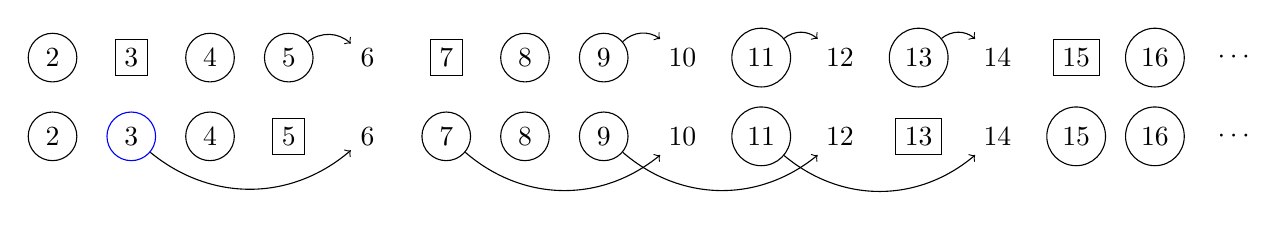
\begin{tikzpicture}
\fill node[circle,draw=black] (1-2) {2};
\fill node[draw, right of=1-2] (1-3) {3};
\fill node[circle,draw=black, right of=1-3] (1-4) {4};
\fill node[circle,draw=black, right of=1-4] (1-5) {5};
\fill node[right of=1-5] (1-6) {6};
\fill node[draw, right of=1-6] (1-7) {7};
\fill node[circle,draw=black, right of=1-7] (1-8) {8};
\fill node[circle,draw=black, right of=1-8] (1-9) {9};
\fill node[right of=1-9] (1-10) {10};
\fill node[circle,draw=black, right of=1-10] (1-11) {11};
\fill node[right of=1-11] (1-12) {12};
\fill node[circle,draw=black, right of=1-12] (1-13) {13};
\fill node[right of=1-13] (1-14) {14};
\fill node[draw, right of=1-14] (1-15) {15};
\fill node[circle,draw=black, right of=1-15] (1-16) {16};
\fill node[right of=1-16] {$\cdots$};

\draw[->, bend left=40] (1-5) to (1-6);
\draw[->, bend left=40] (1-9) to (1-10);
\draw[->, bend left=40] (1-11) to (1-12);
\draw[->, bend left=40] (1-13) to (1-14);

\fill node[circle,draw=black, below of=1-2] (2-2) {2};
\fill node[circle,draw=blue, right of=2-2] (2-3) {3};
\fill node[circle,draw=black, right of=2-3] (2-4) {4};
\fill node[draw, right of=2-4] (2-5) {5};
\fill node[right of=2-5] (2-6) {6};
\fill node[circle,draw=black, right of=2-6] (2-7) {7};
\fill node[circle,draw=black, right of=2-7] (2-8) {8};
\fill node[circle,draw=black, right of=2-8] (2-9) {9};
\fill node[right of=2-9] (2-10) {10};
\fill node[circle,draw=black, right of=2-10] (2-11) {11};
\fill node[right of=2-11] (2-12) {12};
\fill node[draw, right of=2-12] (2-13) {13};
\fill node[right of=2-13] (2-14) {14};
\fill node[circle,draw=black, right of=2-14] (2-15) {15};
\fill node[circle,draw=black, right of=2-15] (2-16) {16};
\fill node[right of=2-16] {$\cdots$};

\draw[->, bend right=40] (2-3) to (2-6);
\draw[->, bend right=40] (2-7) to (2-10);
\draw[->, bend right=40] (2-9) to (2-12);
\draw[->, bend right=40] (2-11) to (2-14);
\end{tikzpicture}
\caption{Application of the three Lemmas in a small range.  Circles denote prohibitions of $\Sigma^2$--structures by \Cref{SigmaNonexistenceLemma}, arrows denote $\Sigma^2$--structures constructed by \Cref{SigmaArrowLemma}, and squares denote exceptional $\Sigma^2$--structures constructed by \Cref{SigmaSpecialCaseLemma}.}
\end{figure}

\begin{corollary}\label{LambdasAreFlat}
For $\G$ a formal group over $\Spec \F_2$ with $\height \G \le 2$, the maps $\lambda_2$ and $\lambda_3$ are flat.
\end{corollary}
\begin{proof}
This is a culmination of the above calculations.  As argued at the beginning of our algebraic analysis, it suffices to show just that $\lambda_2^\circ$ is faithfully flat to make the cocnclusion.  Flatness follows by showing that the map is surjective on tangent spaces, which is exactly the content of \Cref{SigmaNonexistenceLemma}, \Cref{SigmaArrowLemma}, and \Cref{SigmaSpecialCaseLemma}.
\end{proof}

\begin{theorem}\label{MStringTriumvirate}
Let $\G$ be a formal group over a perfect field of characteristic $2$, and assume $\height \G \le 2$.  For $E$ the associated Morava $K$--theory or $E$--theory, there are isomorphisms
\begin{align*}
\Spec E_0 M\String & \xrightarrow\cong \Sigma^3(\CP^\infty_E; \sheaf I(0)), &
\Spec E_0 M\Spin & \xrightarrow\cong C^2_{\mathrm{is}}(\CP^\infty_E; \sheaf I(0)),
\end{align*}
where $C^2_{\mathrm{is}}(\CP^\infty_E; \sheaf I(0))$ is the subscheme of $C^2(\CP^\infty_E; \sheaf I(0))$ consisting of those \textit{inverse-symmetric} functions satisfying $f(x, y) / f(-_{\G} x, -_{\G} y) = 1$.  Moreover, the $E_0$--points of these schemes biject with ring spectrum maps $M\String \to E$ and $M\Spin \to E$ respectively. \qed
\end{theorem}
\begin{proof}
Our goal all along was to use the algebraic model to govern the bar spectral sequences 
\begin{align*}
\Tor^{E_* \Spin/SU}_{*, *}(E_*, E_* BSU) & \Rightarrow E_* B\Spin, &
\Tor^{E_* \Spin/SU}_{*, *}(E_*, E_* BU[6, \infty)) & \Rightarrow E_* B\String. \\
\intertext{Our conclusion from \Cref{LambdasAreFlat} is that they are both concentrated on the $0$--line and isomorphic to the respective Hopf algebra quotients}
E_0 BSU \mmod (E_0 \Spin/SU) & \cong E_0 B\Spin, &
E_0 BU[6, \infty) \mmod (E_0 \Spin/SU) & \cong E_0 B\String.
\end{align*}
Our algebraic models furthermore explicitly identify these quotients on homological schemes as those subschemes on which the stated algebraic identities hold.  The final claim of the theorem follows from even-ness and the universal coefficient spectral sequence.
\end{proof}

\begin{corollary}
If $E$ is a finite height Morava $K$-- or $E$--theory considered as an elliptic spectrum, the complex $\sigma$--orientation of \Cref{EllipticSpectraAreOriented} lifts uniquely to a ring map $M\String \to E$.
\end{corollary}
\begin{proof}
A remarkable feature of the canonical cubical structure associated to an abelian variety is that it automatically satisfies the extra condition required to be a $\Sigma^3$--structure.
\citeme{Someone must state this how you want}
\end{proof}

\begin{remark}[{\cite[Theorem 7.2]{HopkinsICMZurich}}]
More generally, the $\sigma$--orientation associated to a elliptic spectrum which either has $1/2 \in \pi_0 E$ or which has $\pi_* E$ torsion--free is supposed to lift through $M\String$.  Flatness in this setting is supposed to be approached via a fiber-by-fiber criterion, but here the grading tricked used above are less visibly helpful in lifting the classical algebraic result to the periodic one we require to make this work.  Rather than pursue this, we will give a sketch of the construction of the $\String$--orientation of $\tmf$ in \Cref{JuvitopTalkSection}, which automatically gives this much stronger result.
\end{remark}

\begin{remark}[{\cite{KLW,StricklandFSKS}}]
A the cohomology formal schemes of a number of other infinite loopspaces related to real $K$--theory admit reasonable descriptions, often even independent of height.  A routinely useful result in this arena is due to Yagita~\cite[Lemma 2.1]{Yagita}: for $k_\Gamma$ the connective cover of the Morava $K$--theory $K_\Gamma$, in the Atiyah--Hirzebruch spectral sequence \[E_2^{*, *} = Hk^* X \otimes_k k_\Gamma^* \Rightarrow k_\Gamma^* X,\] the differentials are given by \[d_r(x) = \begin{cases} 0 & \text{if $r \le 2(p^d - 1)$}, \\ \lambda Q_d x \otimes v_d & \text{if $r = 2(p^d - 1) + 1$} \end{cases}\] where $\lambda \ne 0$ and $Q_d$ is the $d${\th} Milnor primitive.  For instance, this shows that $K_* BO$ decomposes as \[K_* BO \cong K_*[b_2, b_4, b_{2^{d+1}-2}] \underset{K_*[b_{2j}^2 \mid j < 2^d]}{\otimes} K_*[b_{2j}^2].\]  This, coupled to a theorem governing the result of the double bar spectral sequence, powers most of the results of Kitchloo, Laures, and Wilson~\cite[Section 4]{KLW}.  Their stronger results on the connective covers of $BO \times \Z$ are summarized in \Cref{MoravaKthyOfBO}.  The remaining formal scheme $B\String_K$, our prized object, is harder to access by these means: the sequence $(\OS{HS^1}{2})_K \to B\String_K \to B\Spin_K$ is exact in the middle, but neither left- nor right-exact~\cite[pg.\ 234]{KLW}, causing significant headache.  Satisfyingly, their methods also tell us that our analysis fails at higher heights: the formal scheme $\Spin/SU_K$ contains $\coprod_{j \ge 3} (\OS{HS^1[2]}{j})_K$ as a subscheme, and it accounts for the kernel of the map to $B\Spin_K$.  Once $\height \Gamma \ge 3$ is satisfied, this kernel is nonzero.
\end{remark}

\begin{figure}
\begin{center}
\begin{tikzcd}
& \Div_0 \overline \Gamma[2] \arrow{rr} \arrow{ld} \arrow[equal]{dd} & & \Div_0 \overline \Gamma \arrow{ld} \arrow[equal]{dd} \\
\ker \omega \arrow[crossing over]{rr} \arrow{dd} & & B\Spin_K \\
& \Div_0 \overline \Gamma[2] \arrow{rr} \arrow{ld} \arrow[equal]{dd} & & \Div_0 \overline \Gamma \arrow{ld} \arrow[equal]{dd} \\
\SDiv_0 \Gamma[2] \arrow[crossing over]{rr} \arrow{dd} & & BSO_K \arrow[crossing over, "\omega" near end]{rr} \arrow[crossing over, leftarrow]{uu} & & \Gamma[2]^{\sm 2} \\
& \Div_0 \overline \Gamma[2] \arrow{rr} \arrow{ld} \arrow{dd} & & \Div_0 \overline \Gamma \arrow{ld} \arrow{dd} \\
\Div_0 \Gamma[2] \arrow[crossing over]{rr} \arrow{dd} & & BO_K \arrow[crossing over, "\sigma" near end]{rr} \arrow[crossing over, leftarrow]{uu} & & \Gamma[2] \\
& \Div \overline \Gamma[2] \arrow{rr} \arrow{ld} & & \Div \overline{\Gamma} \arrow{ld} \\
\Div \Gamma[2] \arrow{rr} & & (BO \times \Z)_K \arrow{rr} \arrow[leftarrow, crossing over]{uu} & & \underline{\Z}.
\end{tikzcd}
\end{center}
\caption{Presentations of the Morava $K$--theoretic cohomological formal schemes associated to connective covers of $BO \times \Z$.  Each level in the prism is a bi-Cartesian square in the category of formal group schemes, and each level is the fiber of the maps off of the previous level to the Postnikov section.  The formal curve $\overline \Gamma$ is $\HP^\infty_K$, which is the fiber of $\sigma\co \Div_2^+ \Gamma \to \Gamma$, and $\overline \Gamma[2]$ is the fiber of the lift of the endo-isogeny $2\co \Gamma \to \Gamma$ to $\overline \Gamma$.  The map $\sigma$ vanishes on $\Div_0 \overline \Gamma$ and acts by summation on $\Div_0 \Gamma[2]$.  The map $\omega$ vanishes on $\Div_0 \overline \Gamma$ and acts on $\SDiv_0 \Gamma[2] \cong C_2 \Gamma[2]$ by $[a, b] \mapsto a \wedge b$.}\label{MoravaKthyOfBO}
\end{figure}









\todo{remark: Compare with Neil's response at \texttt{http://mathoverflow.net/questions/123958/a-formal-group-law-over-oriented-bordism}.}
\todo{If you managed to get all this to work, you could try to understand the $M\Spin$--orientation of $K_{\Tate}$, as in page 628 of the published AHS.}
\todo{FPFP Example 12.10 claims applications to $BU[2k, \infty)$, but I can't tell what they are.}
\todo{Mention all this work of Gerd.  He has a bunch of papers that are all clustered around these topics.}










